\documentclass[a4paper,11pt]{article}
\usepackage[T1]{fontenc}
\usepackage[utf8]{inputenc}
\usepackage{lmodern}
\usepackage{mathptmx}
\usepackage[margin=2.5cm]{geometry}
\usepackage{makeidx}
\usepackage{setspace}
\usepackage{fancyhdr}
\usepackage{lastpage}
\usepackage{graphicx}
\usepackage{amsmath}
\usepackage{makeidx}
\usepackage[utf8]{inputenc}
\usepackage[spanish]{babel}
\makeindex 
\graphicspath{{../imagenes/}}                                % Setea el path de las imagenes
\pagestyle{fancy}
\fancyhf{}
\renewcommand{\headrulewidth}{0pt}                        % Saca la línea horizontal del borde superior de las páginas
\cfoot{Pág. \thepage \hspace{1pt}}  % Escribe la cantidad de paginas en el pie de página
\makeindex                                                % Crea el índice
\onehalfspacing                                           % Setea un punto y medio de separación entre líneas
\setlength{\parskip}{6pt}                                 % Setea 6 puntos de separación entre párrafos
\renewcommand{\figurename}{Figura}

\usepackage{hyperref} % For hyperlinks in the PDF
\usepackage{csquotes}
\usepackage[backend=bibtex,bibencoding=ascii, style=alphabetic-verb]{biblatex}
\bibliography{bibliografia}

% Paquetes para tener dos figuras verticales
\usepackage{subcaption}
\usepackage{cleveref}
\captionsetup[subfigure]{subrefformat=simple,labelformat=simple}
\renewcommand\thesubfigure{(\alph{subfigure})}
%\setcounter{chapter}{1}

% Agrega un nivel más bajo de seccionamiento, que subsubsection.
\usepackage{titlesec}
\setcounter{secnumdepth}{4}
\titleformat{\paragraph}
{\normalfont\normalsize\bfseries}{\theparagraph}{1em}{}
\titlespacing*{\paragraph}
{0pt}{3.25ex plus 1ex minus .2ex}{1.5ex plus .2ex}


\title{}
\author{}

%Ésto está echo?
%Títulos de capítulo: Arial ó Times New Roman, 14 puntos, negrita.
%Subtítulos dentro de cada capítulo: Arial ó Times New Roman, 12 puntos, negrita (opcional:
%subrayado). (pueden ir numerados).

\begin{document}


  % ############################ INICIO CARATULA ############################

  \begin{titlepage}

    \begin{center}

      \begin{Huge}
        \textbf{Facultad de Ciencias Exactas, Ingenieria y Agrimensura}\\  
      \end{Huge}
      \vspace*{0.5in}
      \begin{huge}
        \textbf{Licenciatura en Ciencias de la Computación}\\
      \end{huge}
      \vspace*{0.5in}
      \begin{LARGE}
        \textbf{Bases de Datos Avanzadas}\\
      \end{LARGE}
      \vspace*{2.0in}
      \begin{Huge}
        \textbf{MONOGRAFÍA}\\
      \end{Huge}
      \vspace*{0.3in}
      \begin{Huge}
        \textbf{Data Warehouse y OLAP}\\
      \end{Huge}
      \vspace*{2.5in}
      \begin{Large}
        \textbf{Integrantes: Javier Bonet, Joel Catacora}\\
      \end{Large}
      \vspace*{0.1in}
      \rule{80mm}{0.1mm}\\
      \vspace*{0.1in}
      \begin{Large}
        \textbf{2015}\\
      \end{Large}

    \end{center}

  \end{titlepage}

  % ############################ FIN CARATULA ############################


  % ############################ INICIO ÍNDICE ############################
  
  \newpage\null\thispagestyle{empty}\newpage
  \maketitle
  \tableofcontents
  \newpage
  
  % ############################ FIN ÍNDICE ############################

  % ############################ INICIO RESUMEN ############################
    \section{Resumen}
  
    El Data Warehouse es una base de datos orientada a un dominio determinado, integrado, no volátil y variable en el tiempo, que ayuda a la toma de decisiones.
    Estos datos se clasifican en dos grandes grupos: dimensiones y medidas, conceptos fundamentales del modelo dimensional. El cual ofrece los esquemas dimensionales
    (esquema estrella, copo de nieve y constelación), para diseñar el Data Warehouse.
    
    Es posible explotar los datos almacenados de diversas formas:
    reportes, Data Mining, Olap, etc. Olap permite la consulta de grandes cantidades de datos de forma eficiente y sencilla, a partir de la utilización de cubos.
    Estos se utilizan de la misma manera que las bases de datos relacionales utilizan tablas.
    Es por ello, que todo el análisis se hace en términos de los cubos.
    
    Se distinguen dos grandes tipos de sistemas Olap: Rolap y Molap, cuya principal diferencia radica en el tipo de base de datos, con el que se implementa el
    Data Warehouse.
  % ############################ FIN RESUMEN ############################

  
  % ############################ INICIO INTRODUCCIÓN ############################  
  
    \section{Introducción}

    Desde que una empresa u organización es creada, ésta comienza a recabar información, de las distintas transacciones que realiza, al relacionarse
    con alguna entidad externa, o información respectiva a movimientos internos, como por ejemplo el ingreso de personal, gastos administrativos,
    etc. (cuando se habla de transacciones se hace referencia, por ejemplo, a la compra de materias primas de la empresa, venta de mercaderías a un tercero,
    etc.). Desde entonces, se utilizó toda esta información para analizarla y comenzar el proceso de toma de decisiones con el fin de generar un
    crecimiento de la entidad. Por ejemplo, luego de un análisis completo de las ventas realizadas en los últimos meses, se decide incrementar la 
    productividad de un determinado producto habiendo llegado a la conclusión de que fue el más vendido.
    
    Un factor de gran importancia es el tiempo, ya que con el paso del tiempo la información almacenada se vuelve cada vez más grande,
    y por ende difícil de analizar. A mediados de los 80' surge el concepto \textit{Data Warehouse}, como solución a éstos problemas,
    en el ámbito de las bases de datos.
    
    En la sección \ref{conceptos_fundamentales}, se abarca esencialmente: las definiciones de Data Warehouse y Data Mart, sus diferencias con OLTP, el modelo dimensional como
    método de diseño del Data Warehouse, y se explica por qué un Data Warehouse es una base de datos temporal.
    
    En la sección \ref{OLAP}, se presentan las distintas características que definen a un producto OLAP (Reglas de Codd, y FASMI), las jerarquías y agregaciones, y
    su uso en la optimización de las respuestas ante una consulta, la representación del cubo OLAP en dos dimensiones (en forma de grilla), las operaciones
    básicas sobre el mismo, y las principales arquitecturas OLAP.
    
    En la sección \ref{estado_arte}, se detallan cuatros temas en investigación relacionados al Data Warehouse:
    \begin{itemize}
      \item El modelo \textit{MultiDim}, como diseño conceptual del Data Warehouse.
      \item El uso de ontologías como base para el diseño del Data Warehouse.
      \item El modelo de meta tablas \textit{Fuzzy Data Warehouse}, que integra conceptos difusos en un Data Warehouse.
      \item Consideraciones respecto a la seguridad y calidad de los datos del Data Warehouse, cuyas fuentes de datos provienen de la web.
    \end{itemize}
    
    Finalmente el sección \ref{conclusiones}, se encuentran las conclusiones.
    
  % ############################ FIN INTRODUCCIÓN ############################


  % ############################ INICIO CONCEPTOS BÁSICOS ############################
    \section{Data Warehouse: Conceptos fundamentales} \label{conceptos_fundamentales}
    
    Se denominada \textbf{Business Intelligence} (BI, inteligencia de negocios), al conjunto de estrategias que integran, por un lado el almacenamiento, y
    por el otro, el procesamiento de grandes cantidades de datos, con el principal objetivo de generar conocimiento y decisiones en tiempo real, mediante 
    el análisis de los datos existentes en una organización o empresa. Por ello, decimos que BI busca lo siguiente:
    
    \begin{center}
      \textit{Dato + Análisis = Conocimiento.}
    \end{center}


    \subsection{Data Warehouse}
    
    El concepto \textbf{Data Warehouse} (DW, almacén de datos), es una solución dentro del campo de inteligencia de negocios.
    A continuación, presentamos dos definiciones de \textit{Data Warehouse}.

    \begin{itemize}
      \item \textbf{Bill Inmon}, uno de los pioneros en el ámbito de los DW, los define en base a las características que éste debe respetar, las mismas son:
      \begin{itemize}
        \item \textbf{Integrado:} Se integran datos provenientes de múltiples fuentes, posiblemente distintas. Como se verá más adelante, el hecho de tener
        en consideración las fuentes heterogéneas es un punto muy importante al momento de obtener información.
        \item \textbf{No volátil:} Una vez almacenados los datos en el DW, la información que éstos representan no debe perderse. Cuando se dice
        ``no debe perderse'', no quita que los datos puedan ser modificados, siempre y cuando se conserve la información del hecho que se representa.
        \item \textbf{Variable en el tiempo:} La información histórica de la organización en cuestión se mantiene en el DW a lo largo del tiempo.
      \end{itemize}
      \item \textbf{Ralph Kimball}, otro autor reconocido en el tema, por su parte plantea a los DW como una simple copia de los datos transaccionales,
      salvo que los mismos deben estar estructurados de forma tal que permitan un simple análisis y una posterior toma de decisiones en base a los
      datos almacenados.
    \end{itemize}
    
    Si el lector se detiene y analiza brevemente estas definiciones, notará que ambas tienen como eje central la idea del DW como el repositorio central
    donde se almacenan todos los datos recopilados. Un enfoque alternativo plantea al DW con una noción más abstracta, en la que éste engloba
    la arquitectura del proceso completo \textit{Bussiness Intelligence}, el cual comprende la
    extracción de la información de las distintas fuentes hasta la etapa en que el usuario final realiza la explotación de los datos para poder ejecutar el
    proceso de toma de decisiones. La arquitectura se puede observar en la Figura \ref{dw_arq} y a continuación se describirán cada
    una de las partes que la componen:

    \begin{figure}
      \begin{center}
        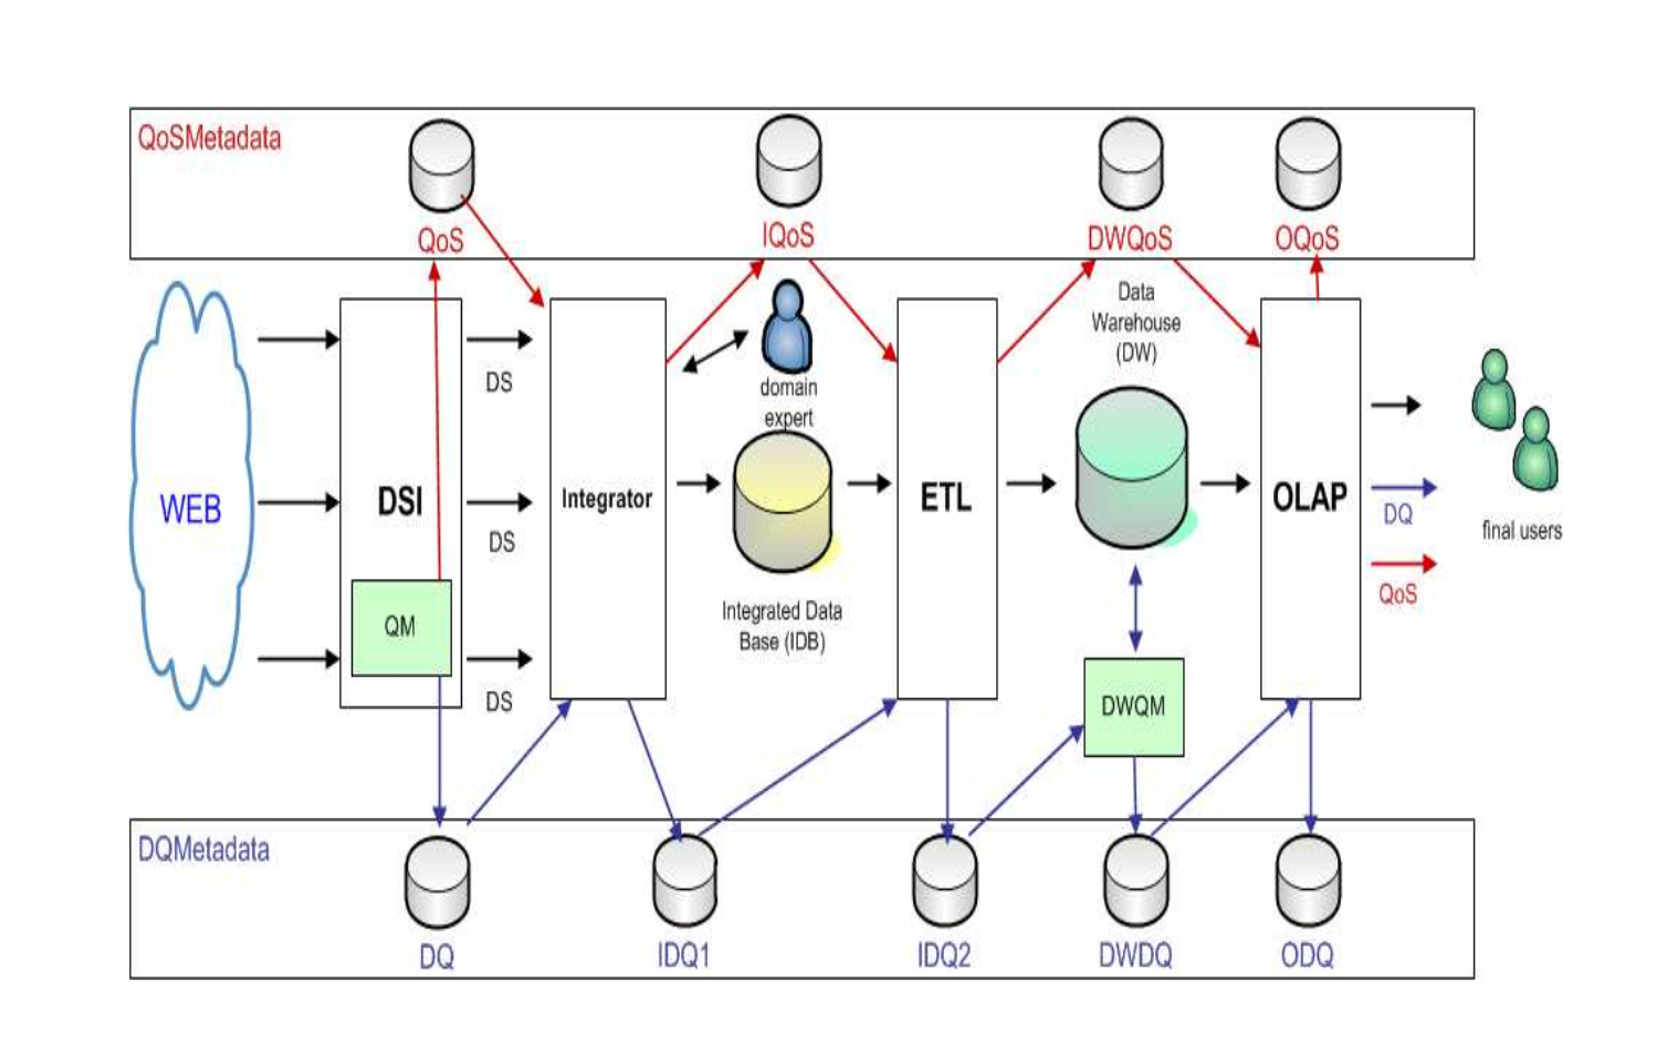
\includegraphics[scale=0.44]{arquitectura}
        \caption{Arquitectura del Data Warehouse}
        \label{dw_arq}
      \end{center}
    \end{figure}
   
    \begin{itemize}
      \item Lo primero que se puede notar en la Figura \ref{dw_arq} son las fuentes de datos, referenciadas en la primera propiedad presentada en la
      definición de Bill Inmon. Las distintas fuentes (posiblemente heterogéneas), son un factor a tenerse en cuenta cuando los
      datos son extraídos. Por ejemplo, la fuente de datos A pueden ser archivos planos de texto, la B archivos \textit{excel} y la C una base de datos 
      transaccional.
    
      \item Luego se observa el módulo \textbf{ETL}, acrónimo en inglés de \textbf{Extraction, Transformation and Loading} (Extracción, Transformación y Carga).
      En esta instancia es donde se aplican diversas técnicas para extraer la información obtenida de
      los diversos orígenes de datos. Luego, se realizan variadas transformaciones (dependiendo de la realidad en que se
      trabaja) para depurar e integrar los datos para cargarlos en un único repositorio central, con el fin de que en posteriores etapas se pueda obtener
      la información de forma sencilla y conociendo una única realidad. (se hace énfasis en esto último debido a que pueden darse situaciones de
      inconsistencia en los datos. Por ejemplo, 2 sectores de la empresa en cuestión informan valores distintos para la venta de un producto en el mismo
      período de tiempo).
    
      \item Seguido al módulo de ETL se observa el repositorio central donde se almacenan los datos depurados y listos para ser explotados utilizando
      diferentes técnicas. Si bien las que aparecen en la Figura \ref{dw_arq} son \textbf{OLAP} y \textbf{Data Mining}, existen muchas otras formas de 
      explotación, sobre las cuales no se entrará en detalles. Por ejemplo, construcción de reportes operativos, tableros de control, etc.
    \end{itemize}

    Todos y cada uno de los pasos, módulos y técnicas a los que se hicieron referencia al explicar la arquitectura de DW tienen como finalidad
    proveer de métodos y procedimientos sencillos con los cuales el usuario final pueda consultar la información almacenada, sin ningún conocimiento técnico y,
    además, pueda obtener la que le sea de utilidad para llevar a cabo un proceso de toma de decisiones simple y con mayor respaldo.
    
    
    \subsection{OLTP}
    
    Estas siglas componen el acrónimo de \textit{OnLine Transaction Processing} (Procesamiento de Transacciones En Línea). Es un tipo
    de procesamiento que facilita y administra aplicaciones transaccionales, usualmente para entrada y recuperación de datos y procesamiento de
    transacciones.
    Las aplicaciones OLTP tienen un alto rendimiento en la inserción o actualización intensiva de una base de datos. Estas aplicaciones son utilizadas
    simultáneamente por centenares de usuarios. Además, tienen como objetivos clave la disponibilidad, velocidad, concurrencia y recuperación.
    Por ejemplo, la aplicación que gestiona a determinado cajero automático de un banco, al tener que estar constantemente actualizando registros de una
    base de datos debido a las repetitivas operaciones de depósitos o giros bancarios, es un claro ejemplo de una aplicación de procesamiento de
    transacciones comerciales.
    En definitiva, los sistemas OLTP son bases de datos orientadas al procesamiento de transacciones, entendiéndose una transacción como un proceso
    atómico (que debe ser validado con un commit, o invalidado con un rollback), y que puede involucrar operaciones de inserción, modificación y
    borrado de datos.\par
    
    En la Figura \ref{oltp_vs_olap} se establece una comparación entre DW y OLTP, que considera los siguientes aspectos:
    
    \begin{figure}
      \begin{center}
        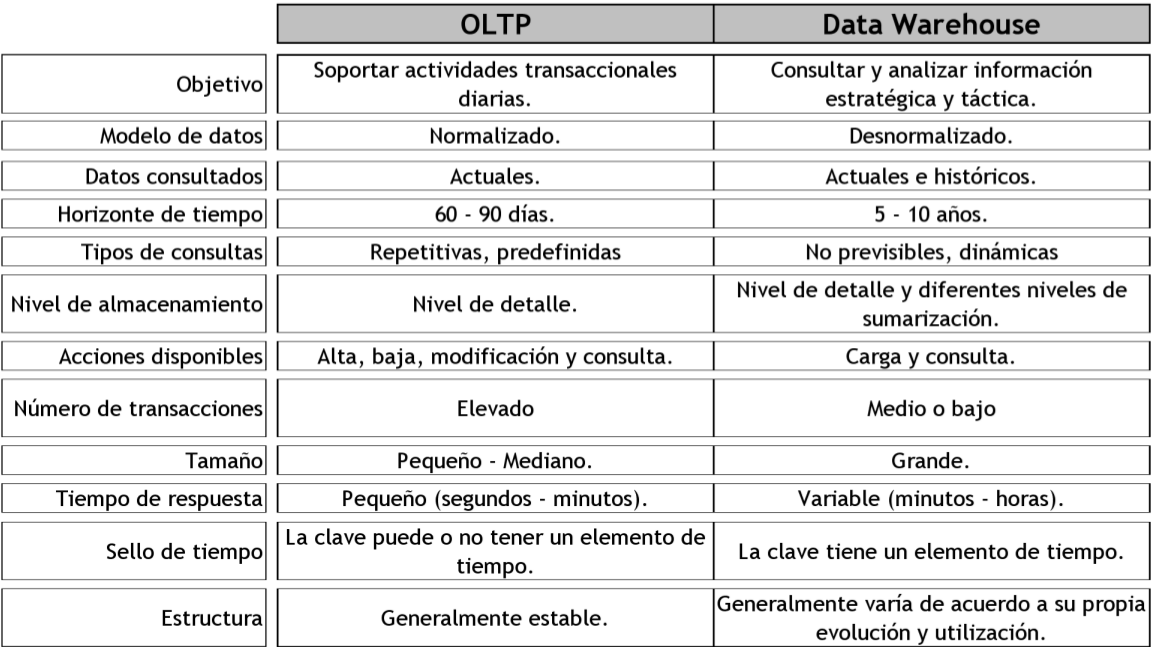
\includegraphics[scale=0.39]{OltpVSDW3}
        \caption{Cuadro comparativo entre OLTP y DW. \cite[p.~42]{hefestov2}.}
        \label{oltp_vs_olap}
      \end{center}
    \end{figure}
    
    
    \begin{itemize}
      \item \textbf{Objetivo:} 
        \begin{itemize}
          \item \textbf{Transaccional:} Diseñado para operaciones de negocio en tiempo real.
          \item \textbf{DW:} Orientado a las consultas y al análisis de los datos con el fin de asistir en la toma de decisiones. 
        \end{itemize}
      \item \textbf{Modelo de datos:}
        \begin{itemize}
          \item \textbf{Transaccional:} Normalizado; evita la redundancia de datos, con lo cual se minimiza el espacio de almacenamiento.
          \item \textbf{DW:} Desnormalizado, ya que esto favorece de rendimiento de las consultas, al reducir la cantidad de joins necesarios
          para obtener la información requerida (se sacrifica espacio en disco para obtener este beneficio).
        \end{itemize}
      \item \textbf{Datos consultados}
        \begin{itemize}
          \item \textbf{Transaccional:} Por la calidad de datos almacenados en las bases de datos transaccionales los datos requeridos son actuales.
          \item \textbf{DW:} Como se mencionó en las características de los DW, los datos almacenados son actuales e históricos, con lo cual se pueden
          consultar ambos tipos de datos.
        \end{itemize}
      \item \textbf{Horizonte de tiempo:}
        \begin{itemize}
          \item \textbf{Transaccional:} Tenemos un horizonte relativamente pequeño ya que las bases de datos transaccionales no tienen esta finalidad.
          \item \textbf{DW:} En este caso tenemos una amplia brecha de tiempo sobre la cual se guarda información ya que la misma es de mucho valor para
          la toma de decisiones.
        \end{itemize}
      \item \textbf{Tipo de consultas:}
        \begin{itemize}
          \item \textbf{Transaccional:} Las consultas disponibles pueden estar acotadas.
          \item \textbf{DW:} Tiene consultas impredecibles que acceden a muchas filas por tabla.
        \end{itemize}
      \item \textbf{Nivel de almacenamiento:}
        \begin{itemize}
          \item \textbf{Transaccional:} Se tiene los datos detallados al nivel definido al comienzo de la creación del esquema de la base de datos.
          \item \textbf{DW:} Al mismo nivel que en la base de datos transaccional y con distintos niveles de sumarización, con lo cual se logra un mayor
          rendimiento en el tiempo de respuesta.
        \end{itemize}
      \item \textbf{Acciones disponibles:}
        \begin{itemize}
          \item \textbf{Transaccional:} Alta, baja, modificación y consulta (insert, delete, update y select) son las acciones básicas.
          \item \textbf{DW:} Carga (Alta) y consulta, las bajas y modificaciones no se realizan debido a que queremos preservar la no volatilidad de los
          datos.
        \end{itemize}
      \item \textbf{Número de transacciones:}
        \begin{itemize}
          \item \textbf{Transaccional:} Soporta miles de usuarios de manera concurrente.
          \item \textbf{DW:} Soporta pocos usuarios simultáneamente, en relación a  OLTP.
        \end{itemize}
      \item \textbf{Tamaño:}
        \begin{itemize}
          \item \textbf{Transaccional:} Al almacenar sólo datos actuales, el tamaño de las bases de datos transaccionales suelen tener tamaños pequeños,
          en relación al DW.
          \item \textbf{DW:} Al contrario de las bases de datos transaccionales, al guardar datos históricos el tamaño de estas bases de datos suelen
          tornarse enormes.
        \end{itemize}
      \item \textbf{Tiempo de respuesta:}
        \begin{itemize}
          \item \textbf{Transaccional:} Está optimizada para un conjunto conocido de las transacciones, por lo general son la adición o la recuperación de
          una sola fila, a la vez, por tabla.
          \item \textbf{DW:} Debido al gran volumen de datos puede ocurrir que los tiempos de respuesta sean variables dependiendo de cada caso.
        \end{itemize}
      \item \textbf{Sello de tiempo:}
        \begin{itemize}
          \item \textbf{Transaccional:} Podría tener o no sello de tiempo, aunque para este tipo de bases de datos tener en cuenta el tiempo no es un
          factor decisivo.
          \item \textbf{DW:} Siempre tendremos una marca de tiempo ya que queremos preservar las característica de no volátil y variable en el tiempo.
        \end{itemize}
      \item \textbf{Estructura:}
        \begin{itemize}
          \item \textbf{Transaccional:} Debido a su utilización, la estructura definida en un comienzo no suele cambiar.
          \item \textbf{DW:} Por ser el mundo de los negocios un ambiente que está en constante evolución, se suele modificar la estructura para que capture
          estos cambios y la información siga aportando conocimiento de utilidad para la toma de decisiones.
        \end{itemize}
    \end{itemize}
    
    Debido a que los datos que son de utilidad (para el fin buscado) son los que contienen información histórica, y concluyendo que OLAP es el tipo
    de procesamiento que corresponde a estos datos (lo cual se deduce de la comparación anterior), a continuación se detallan algunas desventajas del
    procesamiento OLTP para clarificar aún más la diferencia entre ambos tipos de procesamiento:
    
    \begin{itemize}
      \item Gran rigidez a la hora de extraer datos, de manera que el usuario tiene que ceñirse a los informes predefinidos que se configuraron en el
      momento de la implementación, y que no siempre responden a sus dudas reales.
      \item Necesidad de conocimientos técnicos. Para la generación de nuevos informes o métricas suele resultar ineludible acudir al departamento técnico,
      solicitando una consulta adecuada para obtener los datos necesarios de la base de datos.
      \item Largos tiempos de respuesta, ya que las consultas complejas de datos suelen implicar la unión de tablas operacionales de gran tamaño, lo que se
      traduce en una incómoda espera que dificulta la fluidez del trabajo.
      \item Deterioro en el rendimiento del sistema de información. Cuando la base de datos consultada, para generar informes o ratios de negocio, es la
      misma que la que soporta el operativo de la empresa, el funcionamiento del sistema puede degradarse hasta afectar y paralizar a todos los usuarios
      conectados.
      \item Falta de integración que implica ``islas'' de datos. Muchas organizaciones disponen de múltiples sistemas de información, incorporados en
      momentos distintos, para resolver problemáticas diferentes. Sus bases de datos no suelen estar integradas, lo que implica la existencia de ``islas''
      de información.
      \item Datos erróneos, obsoletos o incompletos. El tema de la calidad de los datos siempre es considerado como algo importante, pero esta labor nunca
      se lleva al extremo de garantizar la fiabilidad de la información aportada.
      \item Problemas para adecuar la información al cargo del usuario. No se trata de que todo el mundo tenga acceso a toda la información, sino de que
      tenga acceso a la información que necesita para que su trabajo sea lo más eficiente posible. Por ejemplo, en una organización compuesta por
      diferentes sectores A, B y C, una persona del sector A no debería poder acceder la información de los demás sectores ya que la misma probablemente
      no sea de relevancia para los fines que busca.
      \item Ausencia de información histórica. Los datos almacenados en los sistemas operacionales están diseñados para llevar la empresa al día, pero no
      permiten contrastar la situación actual con una situación retrospectiva de años atrás.
    \end{itemize}
    

    \subsection{Data Marts}
    
    \subsubsection{Definición}

    Los \textbf{Data Marts} (DM), son subconjuntos de datos de un \textit{Data Warehouse} para áreas específicas.
    Entre las características de un DM se destacan:
    
    \begin{itemize}
      \item Usuarios limitados
      \item Tiene un propósito específico
      \item Tiene una función de apoyo
    \end{itemize}
    
    Al hablar de un DM se dice que está destinado para un grupo de usuarios determinados ya que (por definición) está orientado a un área específica de la
    organización o empresa. De la misma observación puede entenderse que su propósito es ayudar en la toma de decisiones sobre el área que está enfocado.
    
    \subsubsection{Metodologías de diseño}
    
    \begin{itemize}
      \item \textbf{Top Down:} Como se puede apreciar en la Figura \ref{top_down}, el DW es cargado a través de procesos ETL y luego éste alimenta a los
      diferentes DM, cada uno de los cuales recibirá los datos que correspondan al tema o departamento que traten. Esta forma de implementación cuenta
      con la ventaja de no tener que incurrir en complicadas sincronizaciones de \textit{hechos}, pero requiere una gran inversión monetaria y más tiempo de
      construcción, que la arquitectura \textit{Bottom Up}.
      \item \textbf{Bottom Up:} En la Figura \ref{bottom_up} se ve claramente como los DM se cargan a través de procesos ETL, los cuales suministrarán la
      información adecuada a cada uno de ellos. En muchas ocasiones, los DM son implementados sin que exista el DW, ya que tienen sus mismas 
      características pero con la particularidad de que están enfocados en un tema específico, con lo cual el volumen de datos es mucho menor y, por ende,
      el manejo de los datos es más sencillo. Luego de haber sido creados y cargados todos los DM, se procede a su integración para obtener el
     repositorio central. La ventaja que trae aparejada este modelo es que cada DM se crea y pone en funcionamiento en un corto lapso de tiempo y se
      puede tener una pequeña solución a un costo no tan elevado. Luego que todos los DM estén puestos en marcha, se puede decidir si construir el DW o no.
      El mayor inconveniente está dado en tener que sincronizar los \textit{hechos} al momento de la consolidación del depósito central.
    \end{itemize}
    
    \begin{figure}
      \begin{center}
        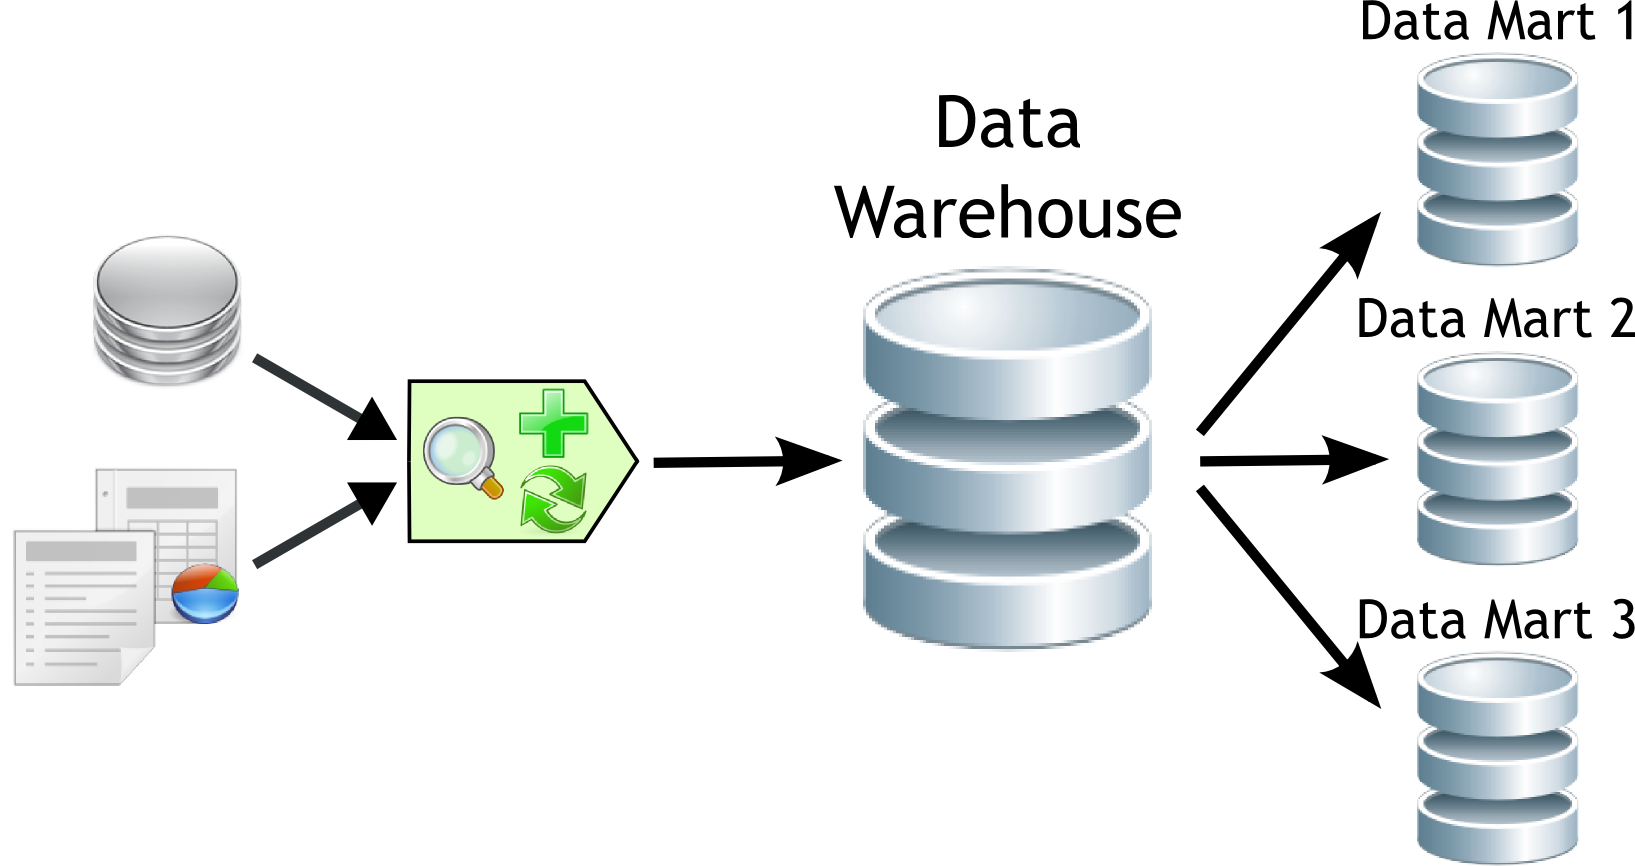
\includegraphics[scale=0.15]{Top-Down}
        \caption{Top Down} \cite[p.~74]{hefestov2}
        \label{top_down}
      \end{center}
    \end{figure}
    
    \begin{figure}
      \begin{center}
        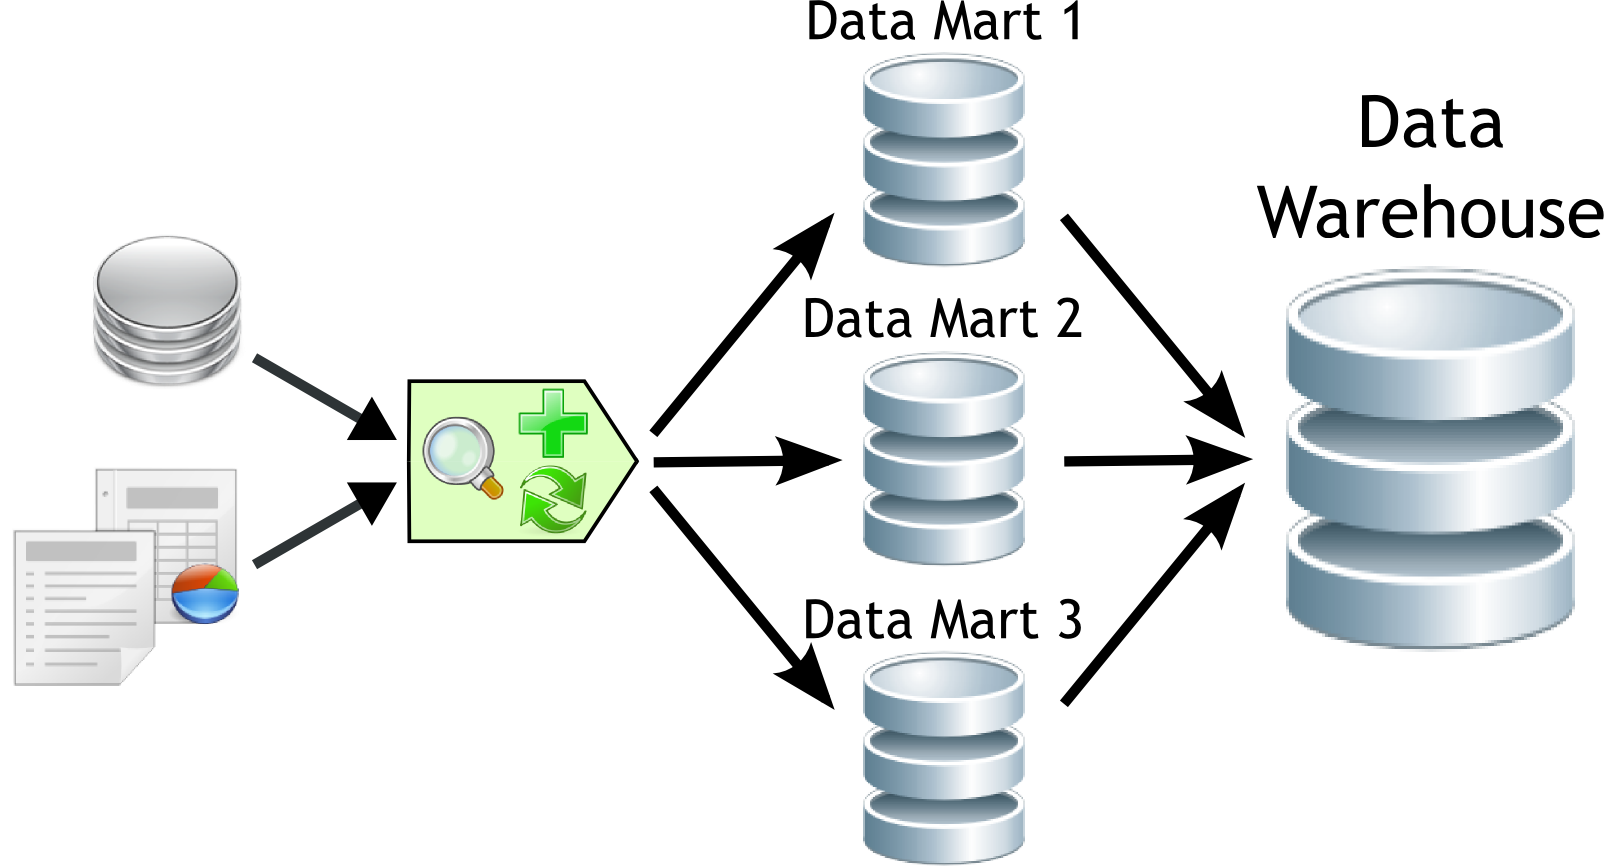
\includegraphics[scale=0.15]{Bottom-Up}
        \caption{Bottom Up} \cite[p.~74]{hefestov2}
        \label{bottom_up}
      \end{center}
    \end{figure}
    
    
    \subsection{Modelo dimensional} \label{mod_dimensional}
    
    El \textbf{modelado dimensional o multidimensional}, es una técnica de diseño lógico de una base de datos, útil para el procesamiento OLAP, que tiene
    como ideas centrales el rendimiento y la comprensión, por parte de los usuarios, de los datos en forma sencilla.
    
    Los conceptos fundamentales del modelo dimensional son:
    
    \begin{itemize}
      \item \textbf{Hechos:} Son las medidas de negocios (o indicadores de negocios) que el usuario final quiere observar y sobre los cuales quiere tener
      conocimientos.
      \item \textbf{Dimensiones:} Éstas son las características que le dan contexto a lo que se quiere observar (hechos).
      Las dimensiones contienen datos cualitativos. Por ejemplo, si uno quiere observar el hecho total 
      vendido, las posibles dimensiones que le dan contexto a esta métrica son el tiempo, el negocio y la ciudad en que se ubica. Si bien cada dimensión hace
      referencia a un concepto específico aportando el contexto en el que se quiere observar el hecho, éste puede estructurarse con un orden jerárquico.
      Por ejemplo, si tenemos una dimensión país, dentro de la misma podríamos tener provincia y ciudad como dos niveles de granularidad. 
    \end{itemize}
    
    \subsubsection{Esquema dimensional}
    
    Se sabe que la relación entre todas las tablas de una base de datos se denomina \textit{esquema de base de datos}. Para un cierto grupo de bases de datos, en las
    cuales se realizan consultas sobre datos históricos, generalmente se utilizan diseños llamados \textbf{esquemas dimensionales}. Un esquema dimensional,
    basado en los fundamentos del modelado dimensional, separa físicamente las medidas que cuantifican el negocio (hechos) de los elementos que los describen
    (dimensiones). Este puede ser de dos tipos:
    
    \begin{itemize}
      \item \textbf{Físico:} Generalmente los objetos que contienen son en realidad tablas de una base de datos, gestionada por una tecnología específica.
      \item \textbf{Lógico:} Los hechos y las dimensiones se representan como entidades y atributos independientes de base de datos en particular,
      y por lo tanto, se pueden transformar en un esquema dimensional físico para cualquier base de datos.
    \end{itemize}
    
    \subsubsection{Tipos de esquemas lógicos}
    
    \paragraph{Esquema de estrella}
  
    Una posible representación relacional del modelo multidimensional esta dado por el esquema estrella.
    Este tipo de esquema tiene una tabla de hechos, rodeada de tablas de dimensiones. En la tabla de hechos habrá un campo por cada dimensión, que
    hace referencia a la clave primaria de la misma (a través de la cual se podrá recuperar la información necesaria para cada hecho),
    y un campo por cada métrica que quiera ser evaluada. La combinación de los campos que referencian a las dimensiones forman, generalmente, la clave primaria de la
    tabla de hechos. Por otra parte, cada dimensión tendrá su campo clave y otros campos en los que se almacenan las correspondientes descripciones que son 
    de utilidad en el ambiente de negocios.
    
    Este esquema es ideal por su simplicidad y velocidad para ser usado en \textit{análisis multidimensionales}. Permite 
    acceder tanto a \textit{datos agregados} \footnote{Ver \ref{agregaciones}.}, como de detalle.
    El diseño de esquemas en estrella permite implementar la funcionalidad de una \textit{base de datos 
    multidimensional} utilizando una clásica base de datos relacional (más extendidas que las multidimensionales). Otra razón para utilizar los esquemas en 
    estrella es su simplicidad desde el punto de vista del usuario final. Las consultas son simples, ya que las condiciones y las uniones (Join) 
    necesarias sólo involucran a la tabla de hechos y a las de dimensiones, sin necesidad de que se encadenen uniones y condiciones a dos o más niveles como 
    es usual que ocurra en un esquema \textit{copo de nieve}.
    
    Consideremos el siguiente ejemplo: supóngase que se quiere realizar un análisis sobre el importe ganado por cliente, según el producto y en una fecha
    específica. Una posible representación utilizando un esquema estrella es el que se observa en la Figura \ref{star_sch}.
    
    Cuando se normaliza, se pretende eliminar la redundancia, la repetición de datos y que las claves sean independientes de
    las columnas, pero en este tipo de modelos se busca tener un formato desnormalizado para que al consultar información se requieran de pocos joins para
    poder obtenerla. En el ejemplo de la Figura \ref{star_sch} las tablas se encuentran desnormalizadas. Para apreciar la
    diferencia, en la Figura \ref{normalizado} muestra la tabla de productos normalizada.
    
    \begin{figure}
      \begin{center}
        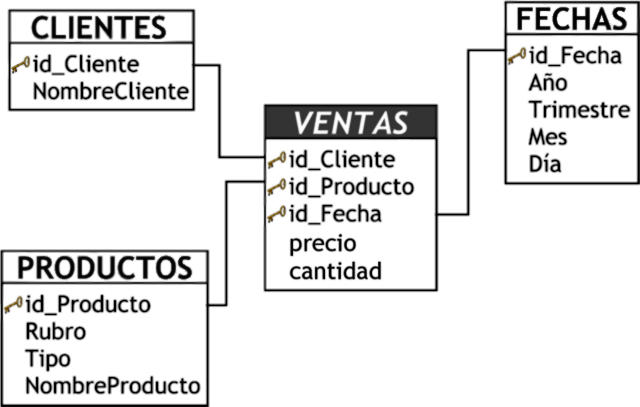
\includegraphics[scale=0.7]{esquema_estrella}
        \caption{Esquema de estrella. \cite[p.~38]{hefestov2}.}
        \label{star_sch}
      \end{center}
    \end{figure}
    
    \begin{figure}
      \begin{center}
        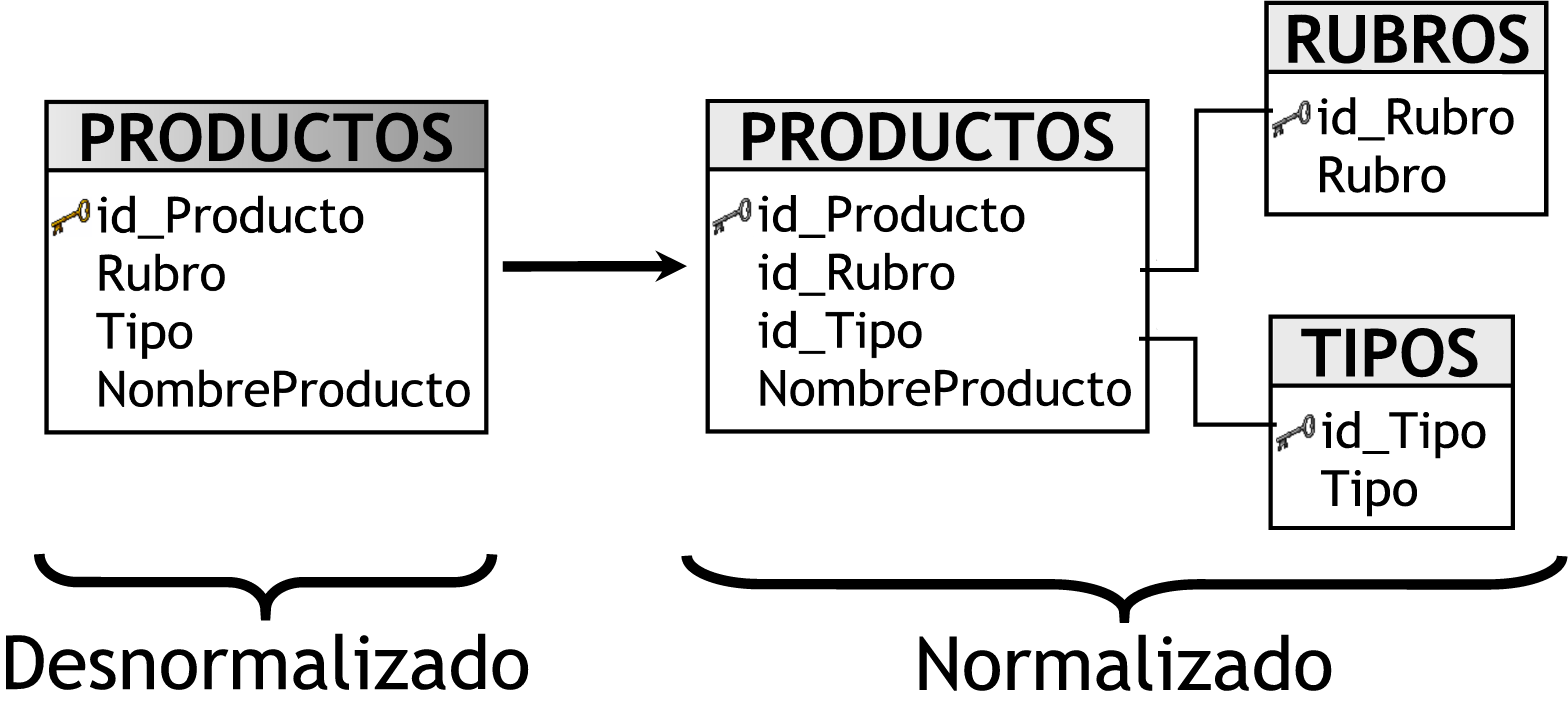
\includegraphics[scale=0.2]{normalizacion}
        \caption{Normalización de Productos. \cite[p.~38]{hefestov2}.}
        \label{normalizado}
      \end{center}
    \end{figure}
    
    
    \paragraph{Esquema copo de nieve}
    
    Este es otro tipo de esquema, similar al esquema de estrella salvo por cierto detalle, las dimensiones pueden, a su vez, estar conectadas con otras 
    tablas de dimensiones. Es decir, habrá una tabla de hechos rodeada de tablas de dimensiones que nuevamente estén conectadas con otras tablas de 
    dimensiones, mediante una relación muchos a uno. Cada una de las dimensiones conectadas con otra dimensión representan un nivel jerárquico para la dimensión en 
    sí misma (por ejemplo, para la dimensión país, podríamos tener una tabla para país, otra para provincia y otra para ciudad). En el ejemplo de la Figura 
    \ref{snow_flk_sch} se ve claramente que una dimensión se implementa con más de una tabla. La razón de esto es buscar la normalización de las tablas, con 
    lo cual se logra reducir espacio de almacenamiento al eliminar redundancia en los datos. Al tener una dimensión (la cual sería representada por una tabla 
    en la base de datos) representada por varias tablas, se facilita su mantenimiento.
    
    Este esquema tiene como finalidad reducir el espacio de almacenamiento, al eliminar la redundancia de datos, pero tiene como contrapartida
    peores rendimientos, en comparación al esquema estrella, al tener que mantener más tablas de dimensiones y más relaciones entre las tablas (Joins).
    
    \begin{figure}
      \begin{center}
        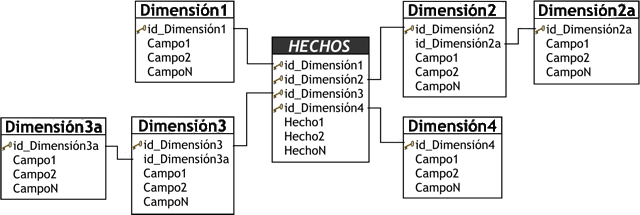
\includegraphics[scale=0.7]{copoNieve}
        \caption{Esquema copo de nieve. \cite[p.~39]{hefestov2}.}
        \label{snow_flk_sch}
      \end{center}
    \end{figure}
    
    
    \paragraph{Esquema de constelación}
    
    Se compone de varios esquemas estrella y/o de copo de nieve. Pueden tener más de una tabla de hechos y compartir dimensiones, entre los hechos.
    La posibilidad de tener más de una tabla de hechos permite que una de ellas sea la principal y las demás contengan diversas sumarizaciones de información
    contenida en la principal.
    
    Este esquema es más complejo que los esquemas anteriores, debido a que contiene varias tablas de hechos. Si bien ésta es una solución flexible, puede 
    llegar a ser difícil de mantener. Puede ser de utilidad en algunos casos donde los hechos están asociados con un nivel de dimensión dada y otros hechos 
    con un nivel más bajo de la dimensión. Un ejemplo sencillo se plantea en la Figura \ref{const_sch} donde se pueden observar 2 tablas de hechos 
    compartiendo dimensiones.
    
    \begin{figure}
      \begin{center}
        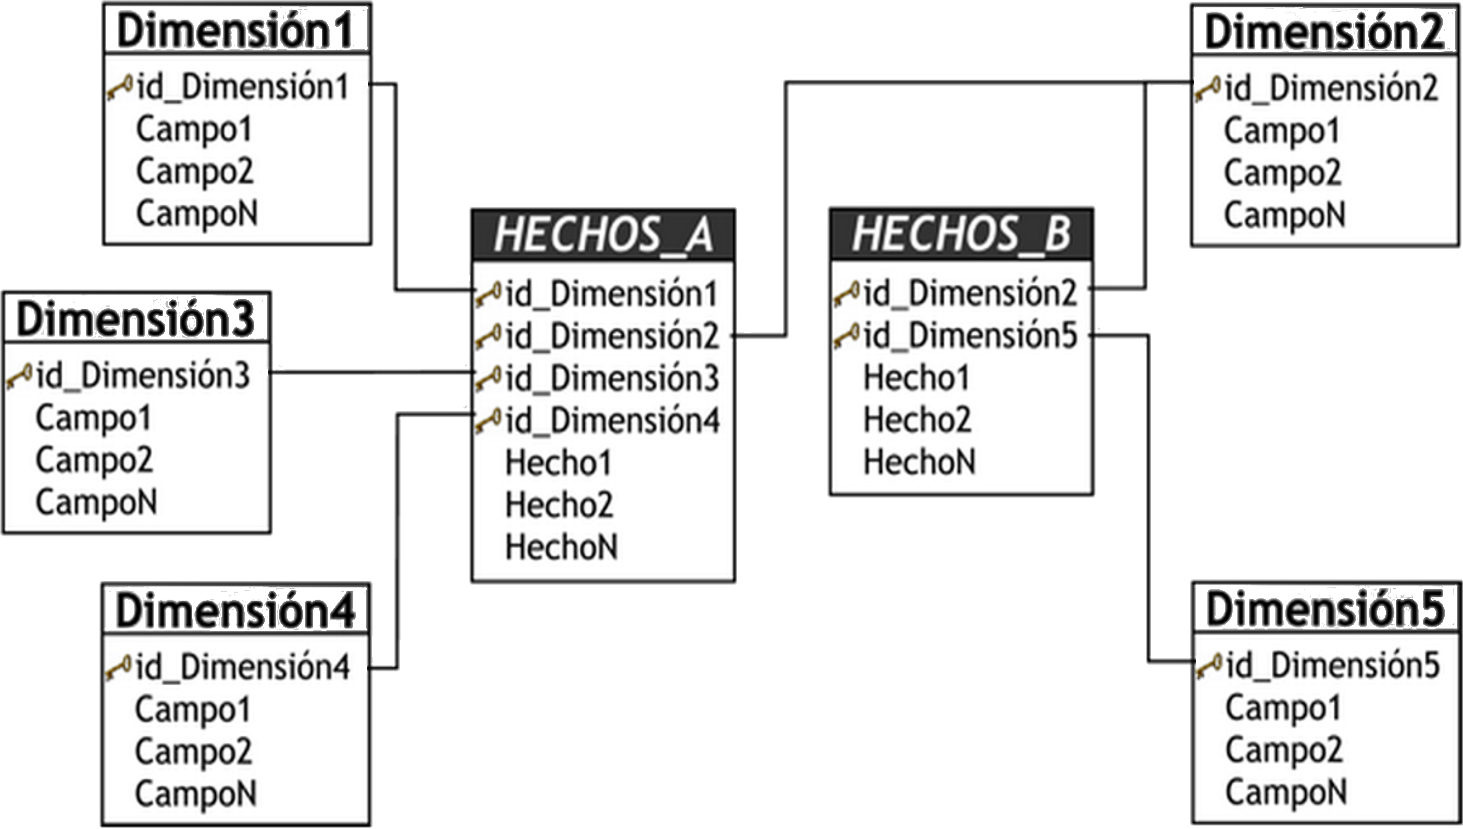
\includegraphics[scale=0.25]{esquema_constelacion}
        \caption{Esquema de constelación. \cite[p.~41]{hefestov2}.}
        \label{const_sch}
      \end{center}
    \end{figure}
    
    
    \subsection{Jerarquías}
    
    Las dimensiones en general, tienen distintos niveles \footnote{Se detalla en \cite[p.~94]{olap_solutions}}, los cuales representan las
    múltiples granularidades de la dimensión (menor o mayor nivel de detalle). Estos niveles forman parte de una jerarquía. El ejemplo más simple de
    jerarquía es el de la dimensión de tiempo, la cual puede ser: \textbf{Año > Mes > Día}. Tanto en la dimensión de
    tiempo como en cualquier otra existe la posibilidad de definir distintas jerarquías. Dos ejemplos sencillos se ilustran en la Figura
    \ref{jerarquías}.
    
    \begin{figure}
      \begin{center}
        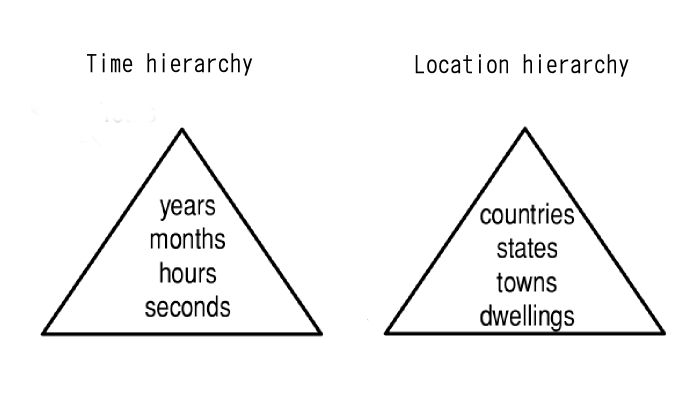
\includegraphics[scale=0.5]{jerarquias}
        \caption{Jerarquías de \textit{Tiempo} y \textit{Ubicación}. \cite[p.~94]{olap_solutions}.}
        \label{jerarquías}
      \end{center}
    \end{figure}
    
    
    \subsection{Agregaciones} \label{agregaciones}
    
    El modelo dimensional permite optimizar el rendimiento de aquellas consultas que requieren solo de datos sumarizados, o de alto nivel,
    mediante la creación de tablas agregadas.
    Un agregado es un resumen precalculado, almacenado por lo general en un esquema separado. Los agregados típicamente se calculan en base
    a los registros en el nivel más detallado (o base) de su jerarquía.
    El número de posibles agregaciones se determina por las combinaciones de las distintas granularidades de cada dimensión.
    Dado que sería muy costoso construir todas las agregaciones  posibles, es una buena idea elegir un subconjunto de tablas sobre las cuales
    hacer agregaciones. La mejor manera de elegir este subconjunto y decidir qué  agregaciones construir, es monitorear las consultas, y diseñar
    las agregaciones que coincidan con los patrones de consulta.
    
    En las Figura \ref{sch_orig1}, se puede apreciar el esquema base sin agregaciones, y en la Figura \ref{sch_agg1} vemos el esquema
    donde los campos tienen un determinado nivel de agregación.
    
    \begin{figure}
      \begin{center}
        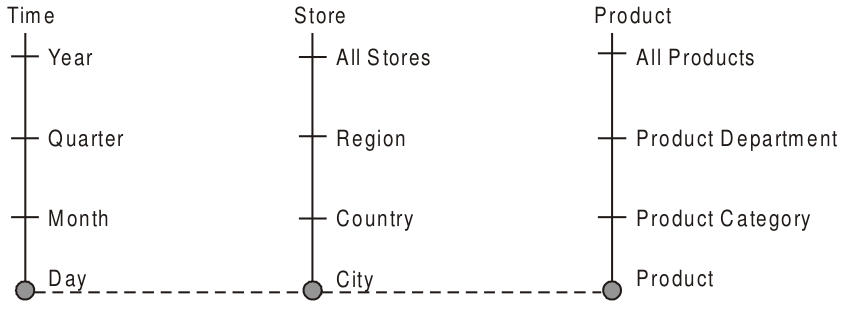
\includegraphics[scale=0.3]{esq_orig1}
        \caption{\textbf{Esquema de nivel base}, contiene los datos en el nivel más detallado. \cite[p.~172]{nagabhushana}.}
        \label{sch_orig1}
      \end{center}
    \end{figure}
    
    \begin{figure}
      \begin{center}
        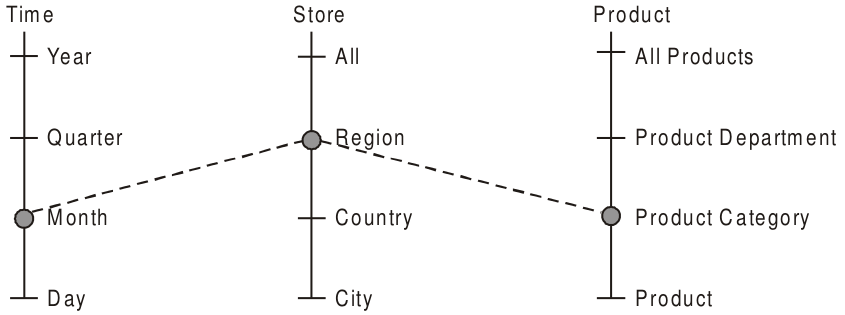
\includegraphics[scale=0.3]{esq_agg1}
        \caption{\textbf{Esquema agregado}, tiene datos en los niveles más alto de las jerarquías. \cite[p.~172]{nagabhushana}.}
        \label{sch_agg1}
      \end{center}
    \end{figure}
    

    Los esquemas agregados proporcionan mejoras en el rendimiento, ya que la cantidad de registros se reduce considerablemente respecto al esquema base. El
    uso más común de los agregados es tomar una dimensión determinada y cambiar su granularidad. Al hacer esto, la tabla de hechos debe ser parcialmente
    resumida para adaptarse a la nueva dimensión. Se crean así, nuevas tablas de dimensión y de hechos, que encajan en el nuevo nivel de granularidad deseado.
    
    En la Figura \ref{sch_orig2} vemos, a modo ejemplo, un esquema copo de nieve con una tabla de hechos y 3 dimensiones.\footnote{Notar que la
    dimensión \textit{Product} está normalizada.} Además, en la Figura \ref{sch_agg2} se puede observar una tabla agregada donde se combinan las tablas de la
    Figura \ref{sch_orig2} de la siguiente forma:
    
    \begin{itemize}
      \item La dimensión de \textit{Time} ``colapsó'' en la tabla de agregación, donde se omitieron los campos \textit{month} y \textit{day}.
      \item Las dos tablas que conforman a la dimensión \textit{Product} colapsaron en la tabla de agregación.
      \item La dimensión \textit{Customer} se dejó de tener en cuenta, en la tabla agregada.
      \item Para cada métrica en la tabla de hechos (\textit{units}, \textit{dollars}) hay una o más métricas en la tabla de 
      agregación (\textit{sum units, min units, max units, sum dollars}).
      \item También se genera una nueva métrica (\textit{row count}) que representa el conteo de las filas.
    \end{itemize}
    
    \begin{figure}
      \begin{center}
        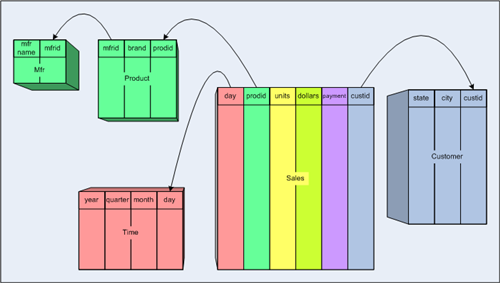
\includegraphics[scale=0.8]{esq_orig2}
        \caption{Esquema original. \cite{agg_tables}}
        \label{sch_orig2}
      \end{center}
    \end{figure}
    
    \begin{figure}
      \begin{center}
        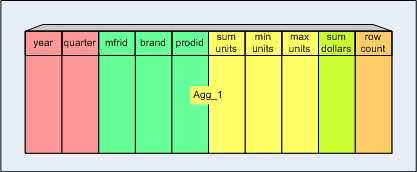
\includegraphics[scale=0.8]{esq_agg2}
        \caption{Esquema agregado. \cite{agg_tables}}
        \label{sch_agg2}
      \end{center}
    \end{figure}
    
    Tener datos agregados en el modelo dimensional hace al entorno más complejo. Para que esta complejidad sea transparente al usuario, se utiliza
    una funcionalidad conocida como \textit{navegación de agregados}, la cual es implementada por el motor OLAP, que permite consultar las
    tablas dimensionales y de hechos, con el nivel de granularidad correcto.
    
    \subsection{Bases de datos temporales}
    
    Una \textbf{base de datos temporal} es una base de datos que trata con especial énfasis aspectos temporales, teniendo un modelo de datos temporal y una versión
    temporal del lenguaje de consulta estructurado.
    
    Los datos almacenados en una base de datos temporal tienen un asociado un período de tiempo que expresa su validez. Las bases de datos convencionales
    consideran que los datos almacenados en ella son válidos, sin importar el tiempo, ya que no mantienen un registro de los estados pasados o futuros de
    la base de datos. En cambio, las bases de datos temporales hacen posible almacenar diferentes estados de la base de datos. Por esto, podemos
    considerar al DW como una base de datos temporal.
    
    
    \subsubsection{Dimensión de tiempo}
    
    En un DW, la creación y el mantenimiento de una tabla de dimensión \textbf{Tiempo} es obligatoria, y la definición de granularidad y estructuración de la misma 
    depende de la dinámica del negocio que se esté analizando. Toda la información del DW, como ya se ha explicado, posee su propio sello de 
    tiempo, el cual determina la ocurrencia de un hecho específico, representando de esta manera, diferentes versiones de una misma situación.Al momento de 
    implementar la dimensión como una tabla en una base de datos se debe tener especial cuidado con el campo clave que se elige ya que esto puede influir 
    mucho en el espacio que se ocupará en disco y los tiempos de respuesta.\par
    
    A continuación se detallan las representaciones más frecuentes del tipo de dato utilizado para la clave:
    
    \begin{itemize}
      \item \textbf{Date:} Si se usa Date como tipo para  el campo clave, costaría mucho espacio en comparación con un entero y los tiempos de respuesta se
      relentizarán ya que para los motores de consulta es más costosa la comparación con este tipo de campos que con uno entero.
      \item \textbf{Entero:}
      \begin{itemize}
        \item Se puede utilizar un campo auto incremental, el cual tiene la siguiente forma: 1, 2, 3, \dots con lo cual el costo de almacenamiento en disco
        se reduciría considerablemente y los tiempos de respuesta bajan ya que la comparación entre enteros no es algo costoso. Sin embargo, con esta representación se
        torna confuso saber con qué fecha se está trabajando.
        \item Una mejor opción es utilizar un campo de la forma yyyyMMdd, por ejemplo 20150315, ya que se obtienen los mismos beneficios que los planteados
        en el item anterior a lo que se suma una mejor comprensión a la hora de visualizar los registros.
      \end{itemize}
    \end{itemize}
    
    
    \section{OnLine Analytical Processing} \label{OLAP}
    
    Más conocido por su acrónimo OLAP (Procesamiento Analítico En Línea), es una solución utilizada en el campo de la inteligencia de negocios, cuyo 
    objetivo es permitir la consulta de grandes cantidades de datos de forma eficiente y sencilla. Utiliza estructuras multidimensionales (cubos OLAP) que 
    contienen datos resumidos de grandes bases de datos.
    
    Como se explico anteriormente, en una base de datos transaccional, normalmente se estructuran las tablas con un modelo normalizado, lo cual favorece a
    la explotación OLTP, en cambio, las bases de datos configuradas para OLAP utilizan un modelo de datos multidimensional, lo que permite consultas 
    analíticas complejas, con tiempos de ejecución más reducidos, que su contrapartida OLTP.

    Las técnicas OLAP, e incluso OLTP fueron iniciadas por E.F. Codd \footnote{El Dr. Codd fue un investigador de base de datos, muy conocido a partir de la
    década de 1960. Es considerado el inventor del modelo de base de datos relacional en 1969.}, considerado el padre de las bases de datos
    relacionales. Las aplicaciones típicas de OLAP se circunscriben en los siguientes ámbitos: informes de negocio de ventas, marketing, informes de gestión,
    gestión del rendimiento empresarial (BMP), presupuestos y previsiones, informes financieros, etc.
    
    
    \subsection{Reglas de Codd}
    
    En 1993, E.F. Codd \& Associates publicó un informe, encargado por Arbor Software (ahora Hyperion Solutions), titulado ``Providing OLAP to User-Analysts:
    An IT Mandate''.
    En un comienzo Codd definió 12 reglas con el fin de evitar que la visión que él tenía sobre las bases de datos relacionales se perdiera, y con el correr
    de los años se extendieron a 18 \footnote{Se pueden observar en \cite[p.~205]{nagabhushana}}. A continuación se detallan las reglas más importantes 
    para los autores:
    
    \begin{itemize}
      \item \textbf{Visión multidimensional:} Las bases de datos OLAP siguen el modelo dimensional. Por lo tanto, OLAP debe ofrecer al usuario final
      una visión de todas las dimensiones del modelo. Provee la base para el procesamiento analítico mediante un acceso flexible y simple a los datos de la 
      organización o empresa.
      \item \textbf{Manipulación intuitiva de los datos:} Lo que se intenta remarcar con esta regla es que tiene que la navegación de los datos debe ser
      sencilla, para lo cual, la mayoría de las aplicaciones ofrecen el doble click o el \textit{drag and drop} para acceder a los datos.
      \item \textbf{Accesibilidad:} Esto está relacionado con el ítem anterior, salvo que de una forma un poco más abstracta. Lo que plantea es que se
      considera a las aplicaciones OLAP como el middleware (capa intermedia) entre las distintas fuentes de información y el usuario final.
      \item \textbf{Soporte de multi-usuario:} La aplicación OLAP debe soportar accesos concurrentes, lo que conlleva a mantener la integridad y seguridad
      de la misma.
      \item \textbf{Información separada del origen de datos:} Esto hace referencia a lo explicado en la arquitectura de DW, ya que se almacena toda la
      información que se va a analizar en el repositorio central, el cual se encuentra separado las fuentes de datos.
      \item \textbf{Flexibilidad ante valores nulos:} Esto punto se refiere a que ante la presencia de valores nulos (posiblemente por no estar informados)
      se diferencien de los valores en 0, lo cual influye en gran medida en los cálculos matemáticos (por ejemplo, podrían no ser considerados en el cálculos
      de promedios). Por otro lado, se debe ofrecer la posibilidad de excluir estos valores para que solamente se visualicen los valores realmente
      importantes.
      \item \textbf{Rendimiento uniforme:} Sin importar la cantidad de dimensiones ni el tamaño que tenga la base de datos, el rendimiento no debe verse
      afectado significativamente.
      \item \textbf{Dimensiones y niveles de agregación ilimitados:} Técnicamente ningún producto puede satisfacer esta regla ya que no se disponen de
      recursos ilimitados. De todos modos, en general, la cantidad de dimensiones y los niveles de agregación varían dependiendo del negocio u organización.
      Son pocas las aplicaciones que necesitan más de 10 dimensiones y jerarquías con más de 6 niveles. Codd sugiere un máximo de entre 15 y 20 dimensiones.
      En cualquier caso, se debe tener en cuenta que la herramienta que se compre tiene sus limitaciones.
    \end{itemize}
    
    
    \subsection{FASMI}
    
    Las reglas de Codd fueron inadecuadas para detectar ``productos OLAP'', por lo que los investigadores se vieron obligados a crear su propia
    definición. La definición debía que ser simple, memorable e independiente del producto, lo que resultó en la prueba FASMI \footnote{Explicada en
    \cite{nagabhushana} Pág. 204.}, Fast Analysis of Shared Multidimentional Information (Análisis Rápido de Información 
    Multidimensional Compartida). Cada componente de esta sigla tiene un significado particular y son explicadas a continuación:
    
    \begin{itemize}
      \item \textbf{Rápido:} Los vendedores recurren a una amplia variedad de técnicas para lograr este objetivo, incluyendo formas especializadas de
      almacenamiento de datos, extensos cálculos previos y requisitos de hardware específicos, pero se cree que ningún producto esté aún completamente
      optimizado en cuanto al tiempo de respuesta, por lo que éste punto se encuentra en un estado de desarrollo.
      El OLAP Survey \footnote{Encuesta a través de los principales productos OLAP, durante 5 años (2001 a 2005).} encontró
      que la lentitud de las respuestas a las consultas, son el problema técnico más frecuente en los productos OLAP, claramente muchas implementaciones
      no superan esta prueba.
      \item \textbf{Análisis:} Los productos deben permitir al usuario definir nuevos cálculos \textit{ad hoc} como parte del análisis e informar los datos de la
      forma en que el usuario lo desee, sin requerir conocimientos técnicos. Esto podría incluir características como el análisis de series de tiempo,las
      asignaciones de costos, la conversión de moneda, búsqueda de objetivos, los cambios estructurales multidimensionales ad hoc, y otras funciones que
      dependen de la aplicación.
      \item \textbf{Información:} Se mide la capacidad de los distintos productos en términos de la cantidad de datos de entrada que puede manejar,
      no de cuántos gigabytes utilizan para almacenarlo.
      \item \textbf{Multidimensional:} El tipo de información que se trata concuerda con el modelo dimensional \footnote{Ver \ref{mod_dimensional}.}.
      \item \textbf{Compartida:} No todas las aplicaciones permiten la escritura de datos, pero si lo hace, el sistema debe ser capaz de manejar múltiples
      actualizaciones de manera oportuna.
    \end{itemize}
    
    
    \subsection{Hipercubo de datos}
    
    OLAP utiliza \textbf{hipercubos} o \textbf{cubos}, de la misma manera que las bases de datos tradicionales utilizan tablas.
    Toda la navegación, informes y análisis se hacen en términos de hipercubos.
    Por lo tanto, un ``cubo'' de datos se refiere a una representación multidimensional de los datos en dicha forma (obviamente, sólo en el espacio tridimensional).
    
    En la construcción de cubos OLAP, las tablas de dimensiones contienen atributos (o campos) que se utilizan para restringir y agrupar
    los datos almacenados en una tabla de hechos cuando se realizan consultas sobre dichos datos en un DW o DM. Los datos en las dimensiones son parámetros
    de los que dependen otros datos que serán objeto de estudio y análisis y que están contenidos en la tabla de hechos. Las tablas de dimensiones ayudan a
    realizar un estudio/análisis aportando información sobre los datos de la tabla de hechos, por lo que puede decirse que en un cubo OLAP, la tabla de
    hechos contiene los datos de interés y las tablas de dimensiones contienen metadatos sobre los hechos.

    El camino hacia la comprensión de los hipercubos no pasa a través de la longitud, ancho y alto de un cubo físico, el cubo es una metáfora visual. Hay
    límites naturales con respecto a lo que se puede hacer en una pantalla de dos dimensiones. Esta limitación ha hecho pensar largo y tendido a los
    desarrolladores de software en busca de la forma óptima de representar la información, con más de dos dimensiones, en una pantalla de computadora plana,
    a efectos de su visualización y manipulación.
    
    Utilizaremos el conjunto de datos de la Figura \ref{tab_cube}, para explicar la visualización de un cubo. Se puede observar una basta cantidad de
    métricas \textit{(Sales, Direct Costs, Indirect Costs, Total Costs y Margin)} y una única dimensión (\textit{Month}) que representa la dimensión de tiempo.
    Es importante aclarar que el conjunto de métricas se considera como una dimensión en sí misma, con lo cual hay dos dimensiones en el esquema del ejemplo planteado.
    Este enfoque de \textbf{dimensiones genéricas}, utiliza invariablemente una \textbf{dimensión de hechos}, o \textit{variable}.
    Tratar a los hechos como miembros de una dimensión, implica la creación de una dimensión de datos. 
    
    Al agregarse una tercera dimensión (\textit{Products}) se obtiene un cubo, en el cual cada celda contiene el valor para un un mes,
    un producto y una métrica determinada, como se puede apreciar en la Figura \ref{cube_2}.
    
    \begin{figure}
      \begin{center}
        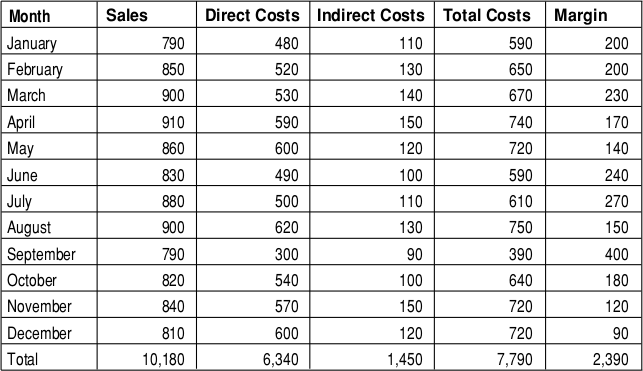
\includegraphics[scale=0.5]{cube_1}
        \caption{Conjunto de datos. \cite[p.~48]{olap_solutions}.}
        \label{tab_cube}
      \end{center}
    \end{figure}
    
    \begin{figure}
      \begin{center}
        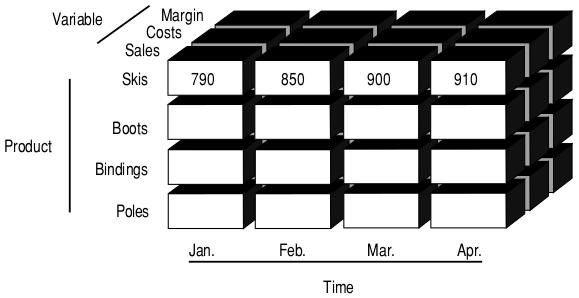
\includegraphics[scale=0.6]{cube_2}
        \caption{Cubo con 3 dimensiones, \textit{Variable, Time, Product}. \cite[p.~49]{olap_solutions}.}
        \label{cube_2}
      \end{center}
    \end{figure}
    
    
    Para representar este cubo tridimensional en una pantalla de dos dimensiones, podemos tomar una ``rebanada'' del mismo.
    Esto consiste en fijar una de las dimensiones (por ejemplo, \textit{Products}) a un valor determinado, con lo cual se obtendrá una
    tabla cuyas celdas contendrán información para los cruces de los valores de las otras dos dimensiones, respecto al producto seleccionado. En la Figura
    \ref{cube_3} se puede observar la visualización del cubo de la Figura \ref{cube_2} habiendo seleccionado el producto \textit{shoes}. Al resultado obtenido se
    lo llama \textit{página} o \textit{rebanada}.
    
    \begin{figure}
      \begin{center}
        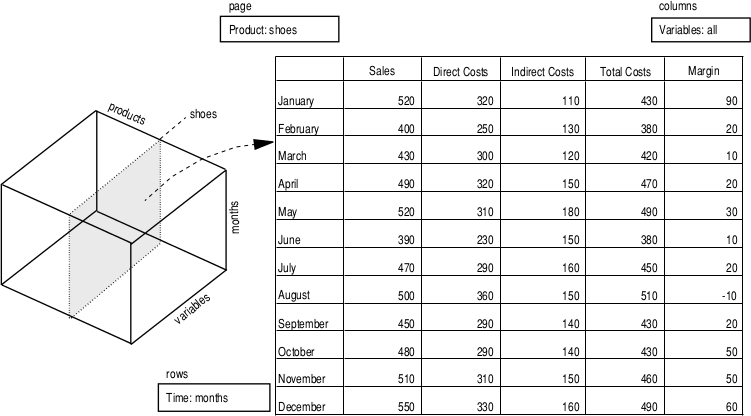
\includegraphics[scale=0.5]{cube_3}
        \caption{Visualización del cubo, mediante una página.} \cite[p.~51]{olap_solutions}.
        \label{cube_3}
      \end{center}
    \end{figure}

    Si se quiere añadir una cuarta dimensión al cubo, el cubo como metáfora visual se rompe; no será posible obtener una visualización del mismo en una
    pantalla de dos dimensiones. Entonces, en \cite{olap_solutions}, se sugiere una nueva estructura para representar los datos, o eventos generadores de datos,
    que es capaz de reproducir cualquier número de dimensiones.
    Se la llama, \textbf{Estructura de Tipo Multidimensional} (\textit{Multidimensional Type Structures}, o MTS).
    Cada dimensión está representada por una línea. Cada miembro dentro de una dimensión está representado por un intervalo, dentro del segmento correspondiente.
    Para el ejemplo presentado en la Figura \ref{cube_2}, tenemos tres líneas:
    Una para el \textit{tiempo}, una de los \textit{productos}, y por último, una para las \textit{variables}.
    Cualquier unión de los intervalos de cada una de los tres líneas, está conectada a un evento y a un elemento del cubo, ver Figura \ref{cube_4}.

    \begin{figure}
      \begin{center}
        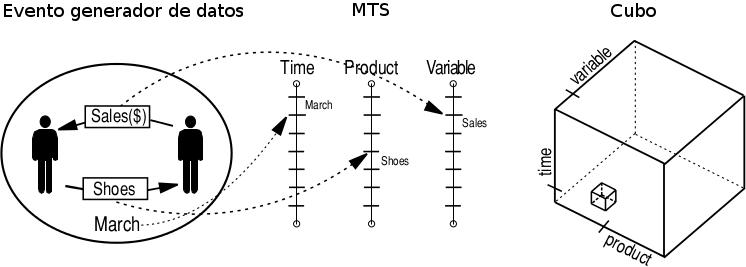
\includegraphics[scale=0.6]{cube_4}
        \caption{Representación de los datos utilizando \textbf{MTS}. \cite[p.~55]{olap_solutions}.}
        \label{cube_4}
      \end{center}
    \end{figure}
    
    
    \subsubsection{Hipercubo en pantalla}
    
    Para lograr que los datos se visualicen en la pantalla de forma correcta, se deberá mapear las múltiples dimensiones lógicas en las dos dimensiones físicas
    que utiliza el monitor.
    Mapear dos dimensiones en una dimensión, implica crear una versión unidimensional de las dos dimensiones.
    El método típico consiste en anidar una dimensión dentro de la otra. En las Figuras \ref{cube_5} y \ref{cube_6} se muestran dos formas distintas en las que
    se puede llevar a cabo éste procedimiento utilizando las dimensiones \textit{Variable} y \textit{Product}.
    
    La Figura \ref{cube_7}, muestra un escenario más elaborado en el que se agregan las dimensiones \textit{Stores} (Tiendas), \textit{Customers} (Tiendas)
    y \textit{Scenarios} (Tiendas). Podemos apreciar el uso del MTS, y múltiples anidamientos, para obtener como resultado final una representación
    bidimensional de las seis dimensiones, en base a filas, columnas y páginas.
    
    \begin{figure}
      \begin{center}
        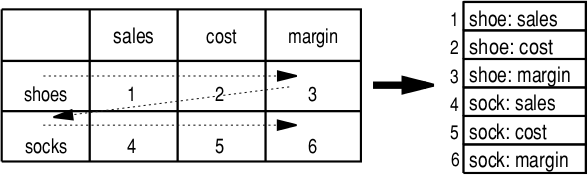
\includegraphics[scale=0.4]{cube_5}
        \caption{Transformación de dos dimensiones a una. Variables anidadas en Productos. \cite[p.~58]{olap_solutions}.}
        \label{cube_5}
      \end{center}
    \end{figure}
    
    \begin{figure}
      \begin{center}
        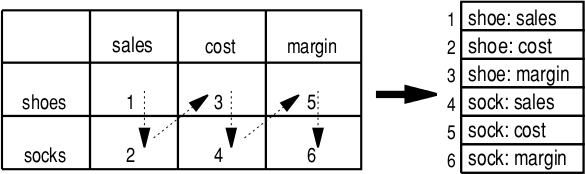
\includegraphics[scale=0.4]{cube_6}
        \caption{Transformación de dos dimensiones a una. Productos anidados en Variables. \cite[p.~58]{olap_solutions}.}
        \label{cube_6}
      \end{center}
    \end{figure}
    
    \begin{figure}
      \begin{center}
        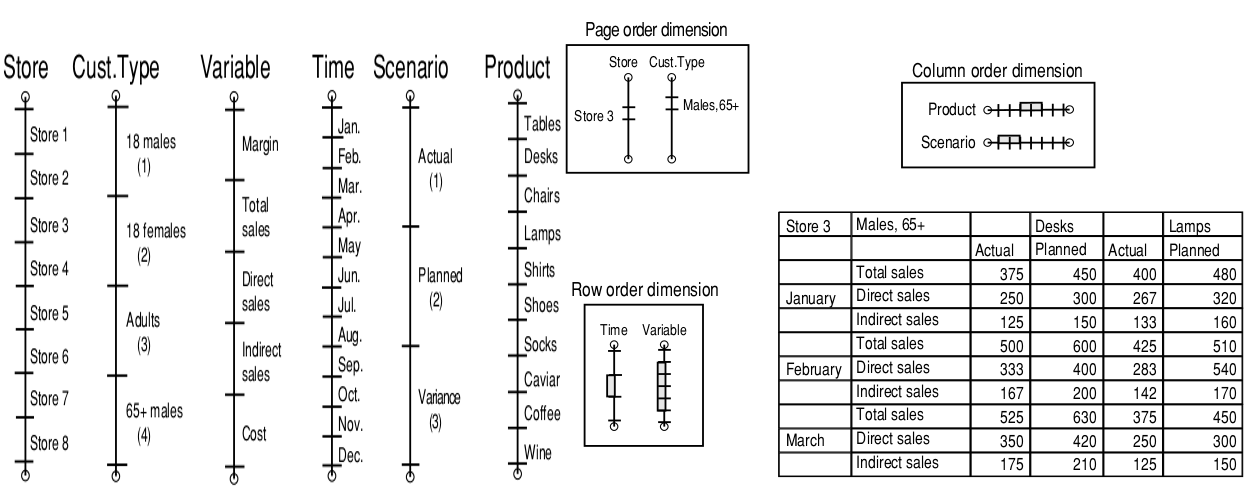
\includegraphics[scale=0.4]{cube_7}
        \caption{Visualización en forma de grilla. \cite[p.~60]{olap_solutions}.}
        \label{cube_7}
      \end{center}
    \end{figure}
    
    
    La capacidad de cambiar fácilmente las vistas de los datos, mediante la reconfiguración de cómo se muestran las dimensiones, es uno de los grandes beneficios
    que proveen los sistemas multidimensionales, lo que es primordial en el momento en que los usuarios finales navegan en busca de información.
    Esto se debe a la separación de la estructura de datos (MTS), de su visualización (grilla).
    
    \vspace{0.2in}
    Para realizar un análisis de los datos multidimensionales, son de mucha utilidad las siguientes reglas básicas:
    
    \begin{itemize}
      \item Tratar de utilizar \textit{páginas}, lo cual permite visualizar la información de mayor relevancia en la pantalla.
      \item Cuando se necesite anidar múltiples dimensiones a través de las filas y columnas, generalmente, es mejor anidar más dimensiones en las columnas que
      a través de filas, ya que las pantallas suelen tener más espacio horizontal que vertical.
      \item Antes de decidir cómo mostrar la información en la pantalla, debe resolver los siguientes interrogantes:
        \begin{enumerate}
          \item ¿Qué se quiere observar?
          \item ¿Qué se intenta comparar?
        \end{enumerate}
    \end{itemize}
    
    
    \subsection{Operaciones sobre el cubo OLAP}
    
    Veremos las operaciones OLAP que los autores consideran más importantes, y junto con las mismas se ilustran
    ejemplos, en base a un cubo de tres dimensiones, \textit{Locations}, \textit{Time}, y \textit{Item}:
    
    \begin{itemize}
      \item \textbf{Slice:} En esta operación se selecciona un valor particular de una de las dimensiones del cubo, buscando con esto obtener una ``rebanada'' del
      mismo. Ver Figura \ref{slice}.
      \item \textbf{Dice:} Se seleccionan valores específicos de dos o más dimensiones, y así se obtiene un subcubo del cubo original. Ver Figura \ref{dice}.
      \item \textbf{Drill Down:} Esta operación ofrece más detalle de la información visualizada, previo a ser aplicada. Esto puede
      lograrse de dos formas, bajar un nivel en la jerarquía de una dimensión en particular o añadir otra dimensión, para sumar aún más información sobre el contexto.
      Ver Figura \ref{drill_down}.
      \item \textbf{Drill up:} En contraposición con la operación anterior, \textit{drill up} permite visualizar menos información, lo cual puede realizarse
      subiendo un nivel en la jerarquía de una dimensión o eliminando alguna de las dimensiones. De ésta forma, se obtiene información con un nivel más alto
      de abstracción. Ver Figura \ref{drill_up}.
      \item \textbf{Pivot:} Ofrece al usuario una presentación alternativa de la información rotando los ejes de datos. Ver Figura \ref{pivot}.
    \end{itemize}
    
    \begin{figure}
        \centering
        \begin{subfigure}[b]{0.5\textwidth}
          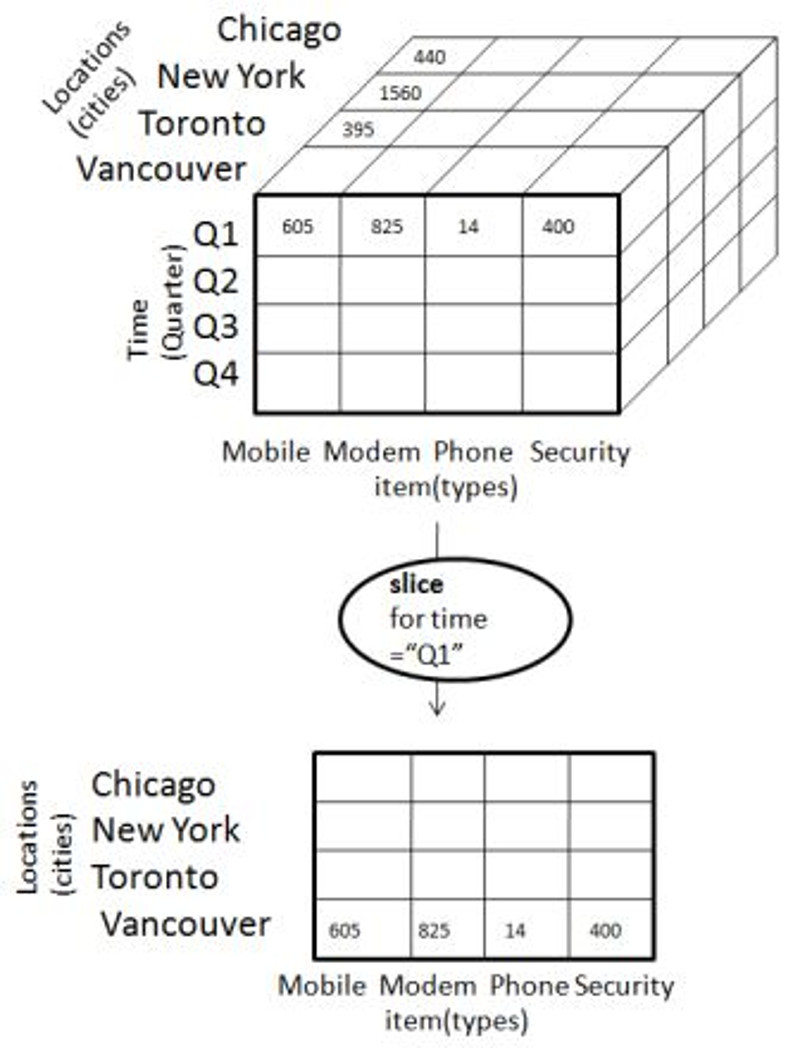
\includegraphics[width=\textwidth]{slice}
          \caption{Operación Slice. \cite{operaciones}}
          \label{slice}      
        \end{subfigure}%
        ~
        \begin{subfigure}[b]{0.5\textwidth}
          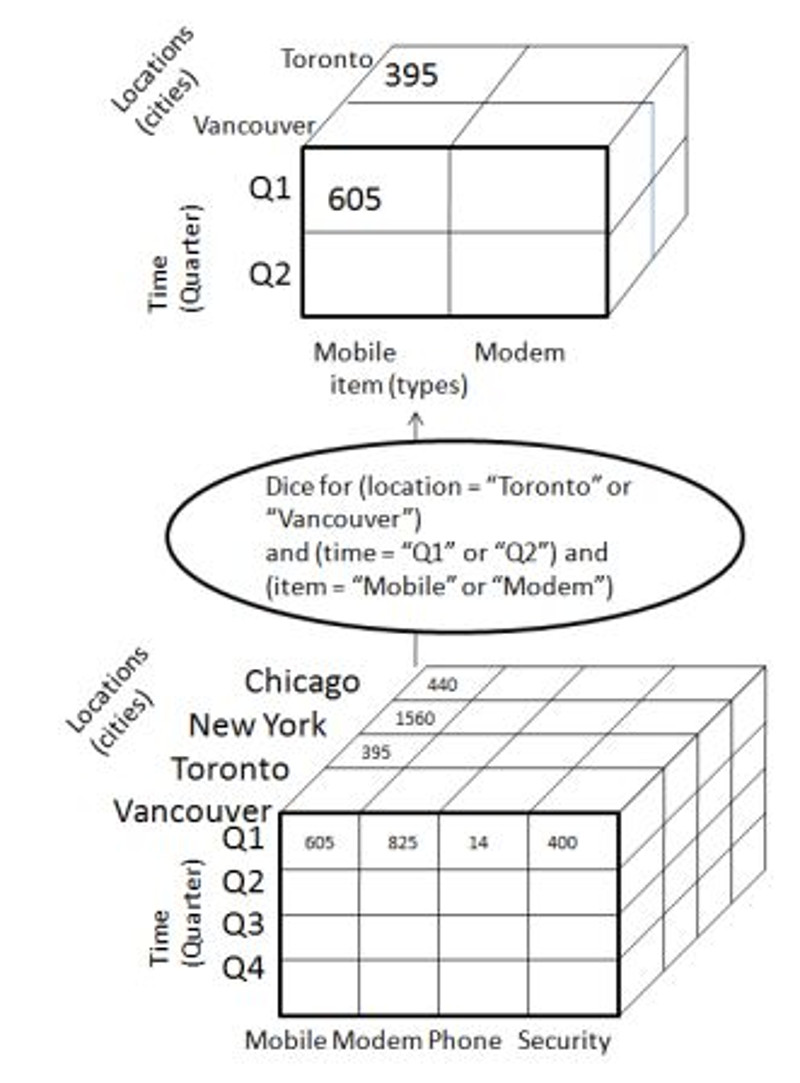
\includegraphics[width=\textwidth]{dice}
          \caption{Operación Dice. \cite{operaciones}}
          \label{dice}
        \end{subfigure}
    \caption{
    \label{slice-dice}%
    Operaciones}
    \end{figure}
      
    \begin{figure}
      \begin{center}
        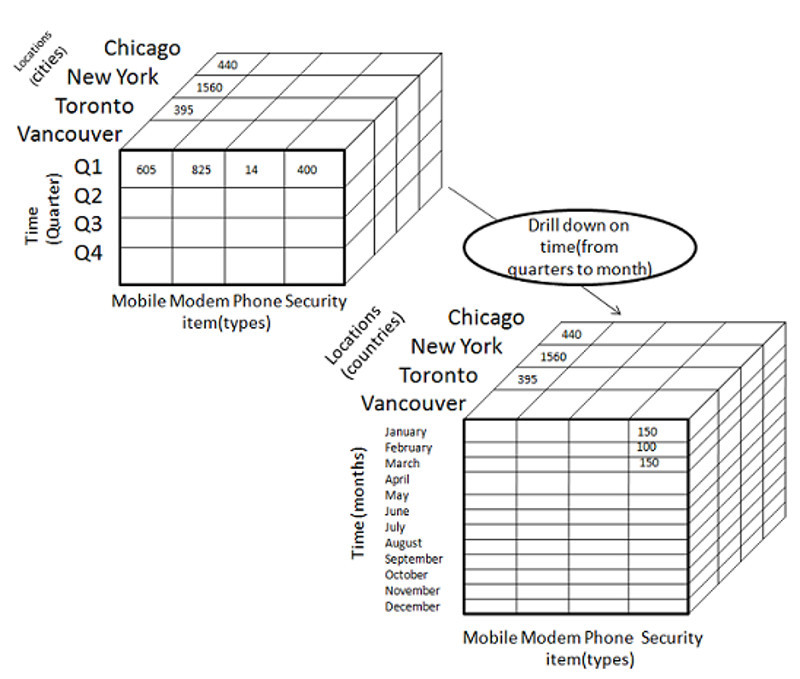
\includegraphics[scale=0.8]{drill_down}
        \caption{Operación Drill Down. \cite{operaciones}}
        \label{drill_down}
      \end{center}
    \end{figure}
    
    \begin{figure}
      \begin{center}
        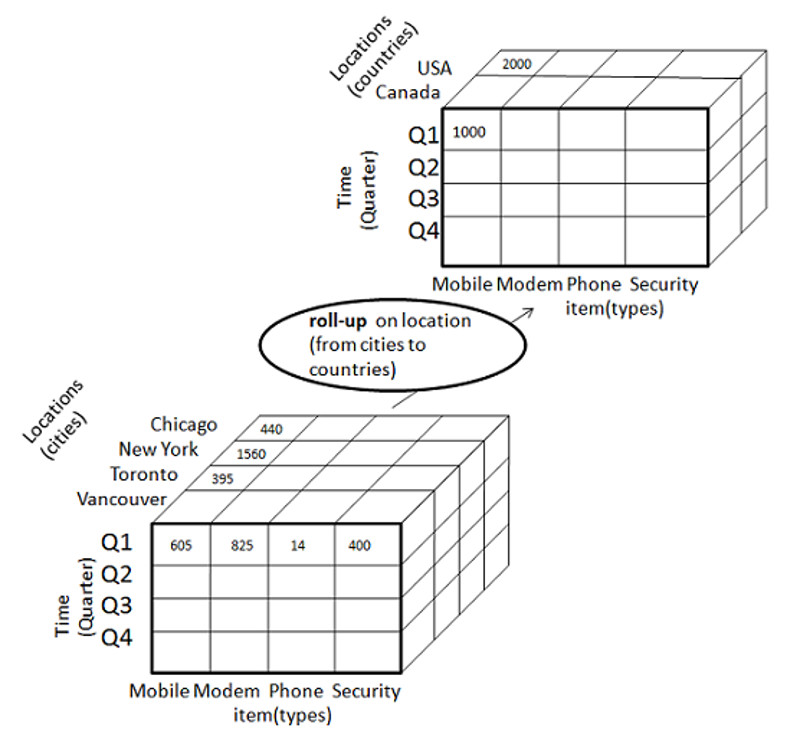
\includegraphics[scale=0.4]{drill_up}
        \caption{Operación Drill Up. \cite{operaciones}}
        \label{drill_up}
      \end{center}
    \end{figure}
    
    \begin{figure}
      \begin{center}
        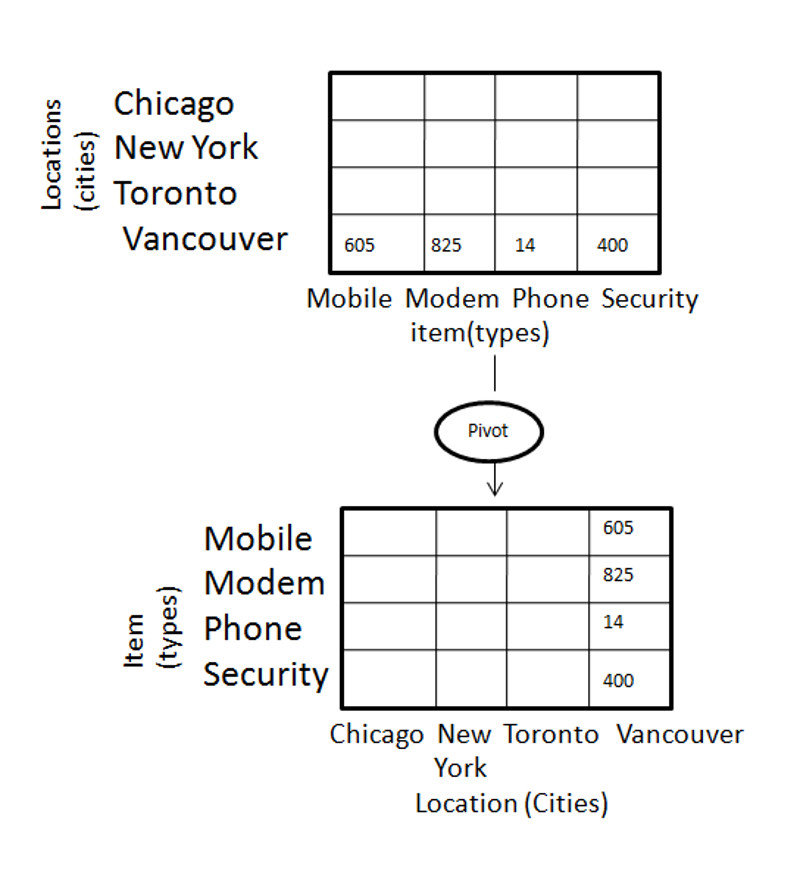
\includegraphics[scale=0.4]{pivot}
        \caption{Operación Pivot. \cite{operaciones}}
        \label{pivot}
      \end{center}
    \end{figure}
    
    
    \subsection{Tipos de OLAP}
    
    \subsubsection{ROLAP}
    
    El \textbf{Procesamiento Analítico Relacional En Línea} (\textbf{ROLAP}, acrónimo de \textit{Relational OnLine Analytical Processing}), consiste en sistemas
    y herramientas OLAP construidas sobre una base de datos relacional. Al trabajar con ROLAP se deben tener en cuenta las siguientes ventajas y desventajas:
    
    \begin{itemize}
      \item \textbf{Ventajas:}
        \begin{itemize}
          \item Existe una gran variedad de herramientas de carga de datos para sistemas relacionales. Con esto se consigue que los tiempos de carga
          sean, generalmente, mucho menores que con las cargas MOLAP (lo cual se definirá a continuación) automatizadas.
          \item Los datos se almacenan en una base de datos relacional estándar que puede ser accedida por cualquier herramienta de generación de
          informes SQL (reporting).
        \end{itemize}
      \item \textbf{Desventajas:}
        \begin{itemize}
          \item Muchos desarrolladores de modelos dimensionales ROLAP ignoran el paso de creación de tablas agregadas, con lo cual el rendimiento de
          una consulta se ve afectado ante la necesidad de consultar las tablas con los datos más detallados. Esto puede evitarse parcialmente
          añadiendo tablas agregadas, sin embargo no es práctico crear tablas agregadas para todas las combinaciones posibles de dimensiones/hechos.
          \item Los sistemas ROLAP se construyen sobre bases de datos de propósito general, por lo que hay algunas funcionalidades especiales, propias
          de las herramientas MOLAP, que no están disponibles en los sistemas ROLAP (tales como el indexado jerárquico especial). Sin embargo, las
          herramientas ROLAP modernas suplen estas carencias con las continuas mejoras del lenguaje SQL, tales como los operadores CUBE y ROLLUP.
          Estas mejoras SQL pueden mitigar en cierto nivel las diferencias frente a las herramientas MOLAP.
          \item Dado que las herramientas ROLAP se basan en SQL para todos sus cálculos, no son apropiadas cuando se realizan muchos cómputos que
          no tienen una traducción simple al SQL (por ejemplo: presupuestos, asignaciones, informes financieros y otros escenarios).
        \end{itemize}
    \end{itemize}
    
    En la Figura \ref{rolap} se puede observar una posible estructura utilizando ROLAP.
    
    \begin{figure}
      \begin{center}
        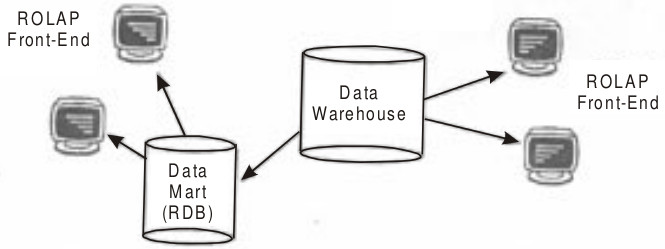
\includegraphics[scale=0.4]{rolap}
        \caption{Estructura de DW utilizando ROLAP. \cite[p.~81]{nagabhushana}.}
        \label{rolap}
      \end{center}
    \end{figure}
    
    \subsubsection{MOLAP}
    
    El \textbf{Procesamiento Analítico Multidimensional En Línea} (\textbf{MOLAP}, \textit{Multidimensional Online Analytical Processing}),
    consiste en herramientas que ejecutan sus cálculos sobre una base de datos multidimensional (MDDB), cual tienen algunas características a favor y otras en contra.
    
    \begin{itemize}
      \item \textbf{Ventajas:}
        \begin{itemize}
          \item Consultas rápidas debido a ciertas optimizaciones de rendimiento, indexación multidimensional y memoria caché.
          \item Ocupa menor tamaño en disco en comparación con los datos almacenados en base de datos relacional debido a técnicas de compresión.
          \item Automatización del procesamiento de los datos agregados de mayor nivel.
          \item Muy compacto para conjuntos de datos de pocas dimensiones.
        \end{itemize}
      \item \textbf{Desventajas:}
        \begin{itemize}
          \item La etapa de procesamiento (carga de datos) puede llevar mucho tiempo, sobre todo para grandes volúmenes de datos. Normalmente, esto se
          puede evitar con un procesamiento incremental, es decir, sólo procesar los datos que han cambiado (por lo general, datos nuevos) en lugar de
          reprocesar todo el conjunto de datos.
          \item Las herramientas MOLAP tradicionalmente tienen dificultades para consultar modelos con muchas dimensiones.
        \end{itemize}
    \end{itemize} 
    
    \begin{figure}
      \begin{center}
        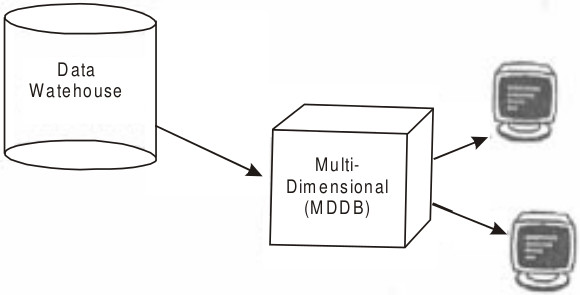
\includegraphics[scale=0.4]{molap}
        \caption{Estructura de DW utilizando MOLAP. \cite[p.~81]{nagabhushana}.}
        \label{molap}
      \end{center}
    \end{figure}
    
    En la Figura \ref{molap} se puede observar una estructura MOLAP.
    
    \subsubsection{HOLAP}

    El coste adicional de los procesos ETL para migrar datos a una herramienta MOLAP y el pobre rendimiento de consulta en los sistemas ROLAP ha generado que la
    mayoría de las herramientas comerciales OLAP usen un modelo \textbf{HOLAP} (\textit{Hybrid OnLine Analytical Processing}), el cual permite al diseñador del sistema
    decidir qué porción de los datos serán almacenados en modo multidimensional (MOLAP) y qué porción en modo relacional (ROLAP). Al combinar ambas herramientas
    se obtiene la reducción de los tiempos que demanda la carga de datos (ROLAP) y las optimizaciones en cálculos complejos, lo que beneficia a la fluidez de la
    navegación de los datos (MOLAP). En la Figura \ref{holap} vemos un modelo HOLAP, donde en una misma arquitectura, conviven ambas tecnologías.
    
    \begin{figure}
      \begin{center}
        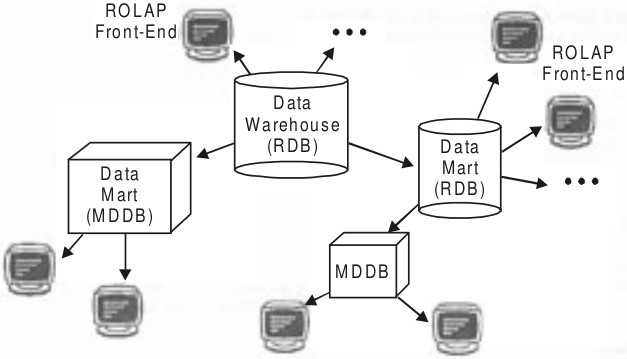
\includegraphics[scale=0.4]{holap}
        \caption{Estructura de DW utilizando HOLAP. \cite[p.~82]{nagabhushana}.}
        \label{holap}
      \end{center}
    \end{figure}

  % ############################ FIN CONCEPTOS BÁSICOS ############################

  % ############################ INICIO ESTADO DEL ARTE ############################
  
    \section{Estado del arte} \label{estado_arte}
    
    En las siguientes secciones se desarrollaran temas que se encuentran actualmente en investigación. Los mismos fueron seleccionados por los autores
    debido a la calidad de información que aportan, y a la relación que se establece entre las bases de datos y temas de la materia
    \textit{Introducción a la Inteligencia Artificial} (lógica difusa, ontologías).
    
    \subsection{Diseño de un Data Warehouse}
    
    El procedimiento, planteado en el libro \cite{VaismanZimanyi14}, se basa en la suposición de que los DWs son un tipo particular de bases de datos dedicada
    a fines analíticos.
    Por lo tanto, su diseño debe seguir las fases de diseño de bases de datos tradicionales, es decir, la especificación de los requisitos, diseño conceptual, diseño 
    lógico y diseño físico. Sin embargo, hay diferencias significativas entre las fases del diseño de bases de una datos tradicional y un DW, que se derivan de su
    diferentes naturalezas. Ver Figura \ref{etapasDiseño}.
    
    A continuación, se detalla cada etapa del diseño de un Data Warehouse, en base a lo recomendado en \cite{VaismanZimanyi14}.
    
    \begin{figure}
      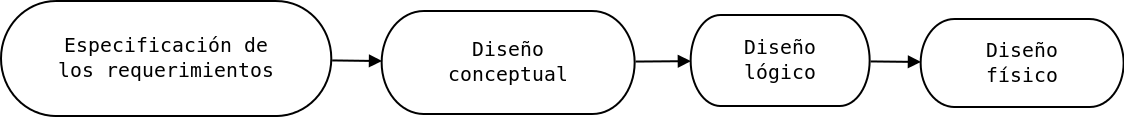
\includegraphics[scale=0.4]{diseno1}  
      \caption{Etapas del diseño de una base de datos.}
      \label{etapasDiseño}
    \end{figure}
    
    \begin{itemize}
      \item \textbf{Especificación de los requerimientos}:
      Determina, entre otras cosas, qué datos deben estar disponibles y cómo deben organizarse. En esta fase, también se determinan las consultas de interés
      para los usuarios. La fase de especificación de requisitos debe conducir al diseñador a descubrir los elementos esenciales de un esquema multidimensional,
      como los hechos y sus dimensiones asociadas, que son necesarios para facilitar la manipulación y cálculos futuros. Esta fase establece una base para todas
      las actividades futuras en el desarrollo del DW; tiene un impacto importante en el éxito del proyecto, ya que afecta directamente a los aspectos técnicos,
      así como las estructuras de almacenamiento de datos y aplicaciones.
      
      \item \textbf{Diseño conceptual}:
      La fase de especificación de requisitos, debe proporcionar los elementos necesarios para la construcción de un esquema conceptual inicial del Data warehouse.
      El objetivo de este esquema es representar los requisitos de una manera clara y concisa, que puedan ser comprendidos por los usuarios. 
      En \cite{VaismanZimanyi14} se propone el modelo \textbf{MultiDim} para definir los esquemas conceptuales, aunque también se pueden utilizar otros modelos
      conceptuales que proporcionen una representación abstracta del esquema del DW.

      Los datos contenidos en los sistemas de origen determina si el esquema conceptual propuesto se puede transformar en esquemas lógicos y físicos, los cuales se
      alimentarán con los datos necesarios para el análisis.
      Todos los elementos incluidos en el esquema conceptual se comparan con los datos en los sistemas de origen.
      Debe especificarse el mapeo de todos los elementos del esquema multidimensional, con los datos en los sistemas de origen. Por ello, el refinamiento del esquema
      conceptual puede requerir varias iteraciones.
      
      \item \textbf{Diseño lógico}:
      Consiste en la transformación del esquema conceptual en un esquema lógico; y segundo, la especificación de los procesos ETL.
      Por lo tanto, es necesario aplicar reglas que mapeen el esquema conceptual con un esquema lógico. Estas reglas de transformación, dependen del modelo conceptual
      utilizado. En \cite{VaismanZimanyi14}, traducen el modelo conceptual MultiDim en el modelo relacional.
      Por lo general, la representación lógica de un DW se basa en el modelo de datos relacional utilizando estructuras muldimensionales específicas, como los esquemas
      estrella y copo de nieve.
      
      \item \textbf{Diseño físico}:
      En ésta fase se deben considerar dos aspectos, la implementación tanto de los esquema del DW, como de los procesos ETL.
      Durante la fase del diseño físico, el esquema lógico se convierte en una estructura de base de datos física.
      Un diseño físico bien desarrollado debiera permitir gestionar grandes cantidades de datos, ya sea para actualizar el almacén de datos con nuevos datos de los
      sistemas de origen, como para realizar operaciones complejas, que pueden incluir joins de muchas tablas, y mantener una gran cantidad de datos.
      \end{itemize}      
      
      \subsubsection{Diseño conceptual: MultiDim}
      
      Un esquema conceptual es una descripción concisa de los requisitos del usuario, sin tener en cuenta los detalles de implementación.
      
      Los esquemas desarrollados mediante el uso de los modelos conceptuales, se puede asignar a varios modelos lógicos, tales como relacionales, objeto-relacional,
      u objeto orientados a modelos, simplificando así las respuestas a los cambios en la tecnología utilizada.
      Por otra parte, los modelos conceptuales facilitan el mantenimiento y evolución de las bases de datos, ya que se centran en los requisitos del usuario;
      en consecuencia, proporcionan un mayor soporte ante posteriores cambios en los esquemas lógicos y físicos.
      
      Sin embargo, en \cite{VaismanZimanyi14} se aclara que no hay un modelo conceptual de datos multidimensionales universalmente aceptado.
      Ante la falta de un modelo genérico, fácil de usar, y comprensible, el diseño del DW, por lo general, se realiza directamente a nivel lógico, en base
      al esquema estrella y/o copo de nieve, lo que genera esquemas difíciles de entender para un usuario típico.
      Proveer de extensiones a E/R y modelos UML para DWs, no son realmente una solución al problema, ya que en definitiva representan
      conceptos de la tecnología relacional subyacentes y, que además, revelan sus propios problemas.
      
      Por lo tanto, se propone el modelo \textbf{MultiDim}, que es lo suficientemente potente como para representar a nivel conceptual
      todos los elementos requeridos en el almacén de datos y aplicaciones OLAP, es decir, dimensiones, jerarquías y hechos asociados a medidas.
      
      \begin{figure}[h]
        \begin{center}
          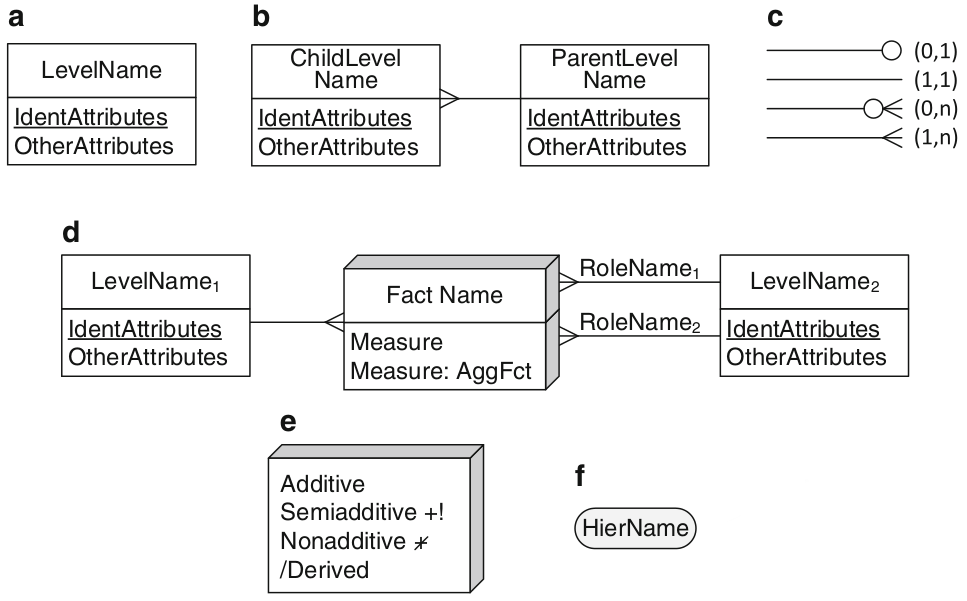
\includegraphics[scale=0.4]{diseno2}
          \caption{(a) Nivel, (b) jerarquía, (c) cardinalidades, (d) hecho con las medidas y niveles asociados, (e) tipos de medidas, (f) nombre de la jerarquía.
          \cite[p.~91]{VaismanZimanyi14}.}
          \label{disenoNotaciones}
        \end{center}
      \end{figure}
      
      A continuación, se detallan las principales componentes del modelo, para más información ver \cite{VaismanZimanyi14}, capítulo 4.
      
      \begin{itemize}
        \item Un \textbf{esquema} se compone de un conjunto de dimensiones y de un conjunto de hechos.
        \item Una \textbf{dimensión} se compone de un nivel o una o más jerarquías.
        \item Una \textbf{jerarquía} está a su vez compuesto por un conjunto de niveles. 
        \item Un \textbf{nivel} es análogo a una entidad en el modelo E/R. En él se describe una serie de conceptos del mundo real que tienen
        características similares. Tiene un conjunto de \textbf{atributos} que describen las características de sus miembros. Además, un nivel tiene uno o
        varios \textbf{identificadores}, que identifican de forma única los miembros de un nivel, cada identificador se compone de uno o varios atributos.
        \item Un \textbf{hecho} relaciona varios niveles. El mismo nivel puede participar varias veces con un hecho, mediante diferentes \textbf{roles}.
        Cada rol se identifica por un nombre. Cada rol se identifica por un nombre y está representado por una relación, entre el nivel correspondiente y el hecho.
        Un hecho puede contener atributos llamados \textbf{medidas}.
        \item Las \textbf{medidas} contienen datos (usualmente numéricos), que son analizados mediante las diversas perspectivas, representadas por las dimensiones.
        Se sumarizan a largo de dimensiones cuando se realizan operaciones roll-up. La \textbf{función de sumarización} asociada
        con una medida se puede especificar junto al nombre de la medida (\textit{SUM}, por defecto). Las medidas pueden clasificarse como sigue,
        de acuerdo a la función de sumarización suma:
        \begin{itemize}
          \item Medidas aditivas: pueden resumirse a lo largo de todas las dimensiones.
          \item Medidas semiaditivas: se pueden resumir, a lo largo de algunas, no todas, las dimensiones.
          \item Medidas no aditivas: no pueden resumirse, través de ninguna dimensión.
        \end{itemize}
        Además, las medidas y los atributos de nivel pueden \textbf{derivarse}, es decir que se calculan en base a otras medidas o atributos en el esquema.
        Por defecto, las medidas son aditivas.
      \end{itemize}
      
      \begin{figure}
        \begin{center}
          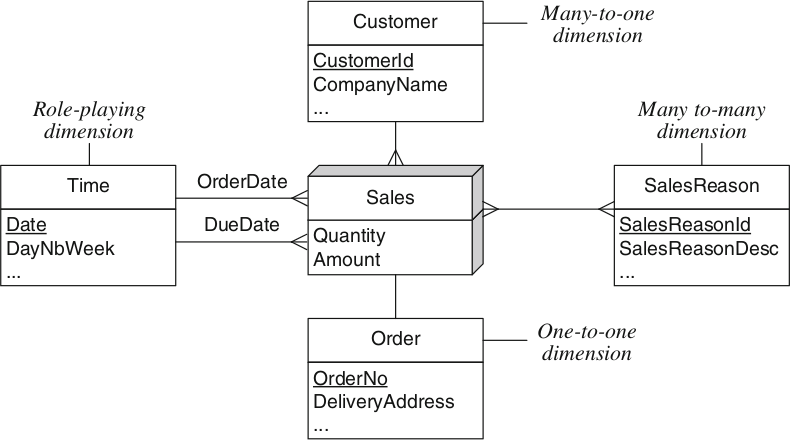
\includegraphics[scale=0.4]{diseno3}
          \caption{Ejemplo. \cite[p.~592]{VaismanZimanyi14}.}
          \label{disenoEj1}
        \end{center}
      \end{figure}
      
      \begin{figure}
        \begin{center}
          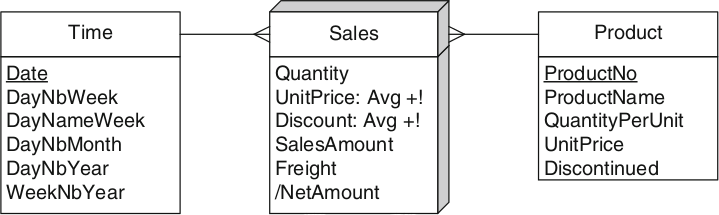
\includegraphics[scale=0.4]{diseno4}
          \caption{Ejemplo. \cite[p.~107]{VaismanZimanyi14}.}
          \label{disenoEj2}
        \end{center}
      \end{figure}
    
      Dados dos niveles relacionados mediante una jerarquía, el nivel inferior se lo llama hijo y el nivel más alto se llama el padre.
      Por lo tanto, las relaciones que componen las jerarquías se denominan relaciones padre-hijo.
      
      Las cardinalidades en las relaciones entre padres e hijos, indican el mínimo y el número máximo de miembros en un nivel que pueden estar relacionados
      con un miembro en otro nivel.
      Una dimensión puede contener varias jerarquías, cada uno expresa un criterio particular, según el fin del análisis; por lo tanto, se incluye el nombre
      de la jerarquía para diferenciarlos. Si un solo nivel contiene atributos que forman una jerarquía, esto significa que el usuario no está interesado
      en el empleo de esta jerarquía.
      
      En la Figura \ref{disenoNotaciones}, se puede ver algunas de las notaciones del modelo MultiDim. Mientras que en la Figuras \ref{disenoEj1} y \ref{disenoEj2},
      se muestra ejemplos que utilizan el modelo.
      
  
    
    \subsection{Ontologías para la creación de un Data Warehouse}
    
    Como se menciona en \cite{ontologias}, la utilización y el análisis de datos no estructurados como pueden ser los archivos de texto, la web
    semántica, etc., han sido incluidos entre las posibles fuentes de datos, debido a la variedad y cantidad de información que pueden aportar. Lo que
    se intenta conseguir es una forma de automatizar la creación de un DW teniendo como base una ontología. Notar que la misma debe tener una
    estructura tal que contenga la información necesaria para la toma de decisiones, con lo cual las distintas clases estarán relacionadas de forma
    que, terminado el algoritmo, se podrán observar las dimensiones y los hechos del DW. Se utilizará como entrada una ontología (escrita en OWL o RDF)
    para luego obtener un DW.\par
    
    Antes de centrar la atención en el algoritmo propiamente dicho, se repasarán algunos conceptos de la teoría de ontologías que resultan fundamentales
    para la comprensión del tema que se analizará en breve:
    
    \begin{itemize}
      \item \textbf{Object Property:} Las propiedades de objetos son relaciones entre instancias de 2 clases. Por ejemplo, ownedBy, podría ser una
      object property con la clase Vehículo como dominio y la clase Persona como rango, la misma establece la relación de pertenencia de un vehículo a
      una persona.
      \item \textbf{Data Property:} Las propiedades de datos son como las object properties pero tienen como dominio una clase y como rango un tipo de
      datos\footnote{Una instancia de una data property relaciona un individuo de la clase dominio con un valor concreto del tipo de datos del rango}.
      Por ejemplo si a una persona se le quisiera asignar el nombre completo, entonces se puede definir la data property fullName con dominio en Person
      y rango string.
      \item \textbf{Individials:} Los individuos de una ontología representan los objetos o instancias de las clases definidas en la misma.
    \end{itemize}
    
    
    Habiéndose presentado las anteriores definiciones, se procederá a detallar el algoritmo en cuestión. El mismo consta de las siguientes etapas:
    
    \begin{itemize}
      \item \textbf{Creación de tablas}
      \item \textbf{Detección de relaciones de subclase}
      \item \textbf{Definir relaciones a partir de propiedad de objetos}
      \item \textbf{Definir relaciones a partir de propiedad de datos}
      \item \textbf{Insertar datos en las tablas}
    \end{itemize} 
    
    \subsubsection{Creación de tablas}
    
    En esta primer etapa el objetivo es que para cada clase en la ontología se deberá crear una tabla en el DW. Es decir, al navegar toda la ontología,
    cada vez que se encuentre una clase, se debe crear una tabla con el mismo nombre en el DW. En la Figura \ref{createTables} se describen, con un
    diagrama de flujo, los pasos a seguir.
    
    \begin{figure}
      \begin{center}
        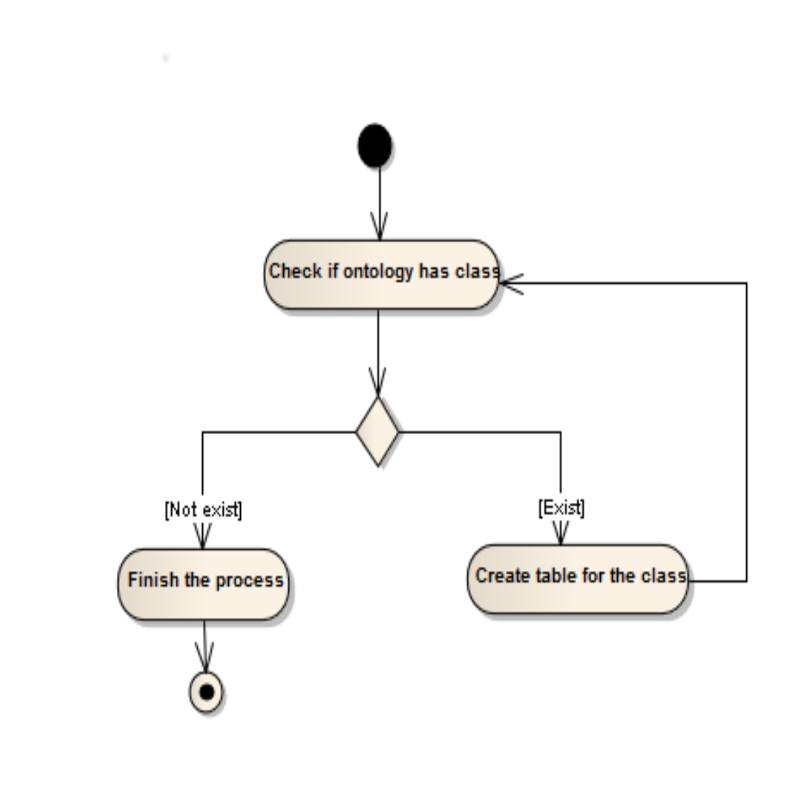
\includegraphics[scale=0.6]{create_tables}
        \caption{\textbf{Primer etapa:} Creación de tablas} \cite[p.~20]{ontologias}.
        \label{createTables}
      \end{center}
    \end{figure}
    
    \subsubsection{Detección de relaciones de subclase}
     
    Ahora se debe centrar la atención en buscar relaciones entre clases del tipo \textbf{subclaseDe}, también conocidas como \textbf{Es\_Un}. Estas
    relaciones expresan que una determinada clase es subclase de otra más abstracta. La subclase hereda todas las propiedades de su clase padre.
    Entonces, cuando se navega toda la ontología y se encuentra este tipo de relación entre dos clases, se tiene que crear una clave foránea (foreing
    key) en la tabla padre y generar una relación uno a muchos entre ambas tablas. Para comprender mejor esta instancia del algoritmo obsérvese la
    Figura \ref{subClase}.
   
    \begin{figure}[!htb]
      \begin{center}
        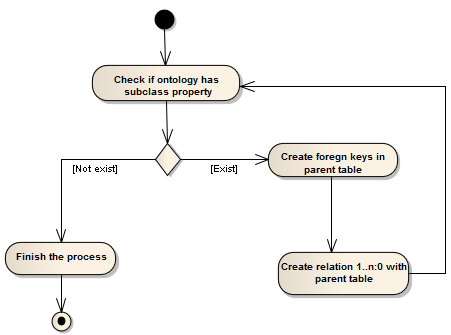
\includegraphics[scale=0.6]{sub_clase}
        \caption{\textbf{Segundo etapa:} Detección de relaciones de subclase} \cite[p.~20]{ontologias}.
        \label{subClase}
      \end{center}
    \end{figure}
     
     
    \subsubsection{Definir relaciones a partir de propiedad de objetos}
    
    Se recorre la ontología en busca de propiedades de objetos. Este tipo de propiedades tienen asociadas un dominio y un rango, los cuales son clase
    (representados con tablas en el DW). Teniendo las tablas dominio y rango, se genera, para cada propiedad de objeto, una relación uno a muchos entre ambas. En
    el caso en que no existan el dominio y el rango (debido a estar tratando con una sub-propiedad), se toma el dominio y el rango de la propiedad padre y se
    realiza el mismo procedimiento. Se puede observar en la Figura \ref{objectProperty} qué pasos son los que se deben realizar para completar correctamente esta
    etapa.
    
    \begin{figure}[!htb]
      \begin{center}
        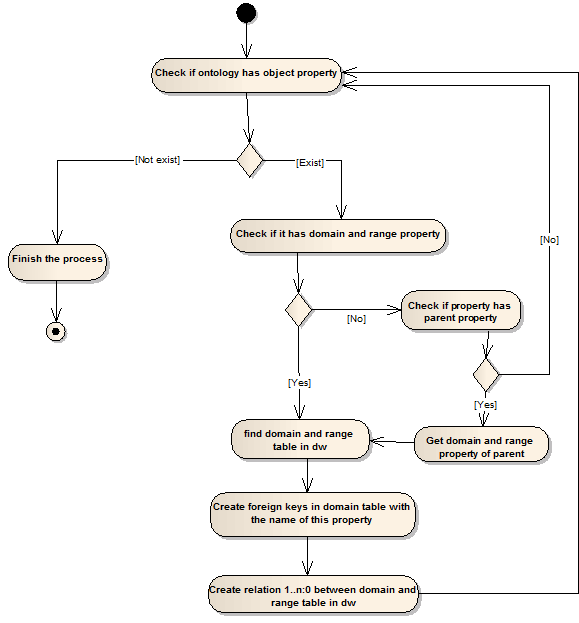
\includegraphics[scale=0.6]{object_property}
        \caption{\textbf{Tercer etapa:} Detección de propiedades de objeto} \cite[p.~21]{ontologias}.
        \label{objectProperty}
      \end{center}
    \end{figure}
    
    
    \subsubsection{Definir relaciones a partir de propiedad de datos}
    
    Se buscan todas la propiedades de datos en la ontología. Las propiedades de datos vinculan una clase con un tipo de dato específico. Similar a las propiedades
    de objetos, las propiedades de datos tienen dominio y rango. Si se puede identificar el dominio y rango de la propiedad, en la tabla que representa al dominio
    creamos una columna con el mismo nombre de la propiedad y seteamos el tipo de esa columna como el rango de la propiedad. En caso que no se pueda encontrar el
    dominio y rango, se debe intentar identificar la propiedad padre de esta propiedad (si existe) y dado el caso, realizamos el mismo procedimiento con el
    dominio y rango de la propiedad padre. Se puede apreciar, en la Figura \ref{dataProperty}, qué es lo que se debe realizar en esta etapa.
    
    \begin{figure}[!htb]
      \begin{center}
        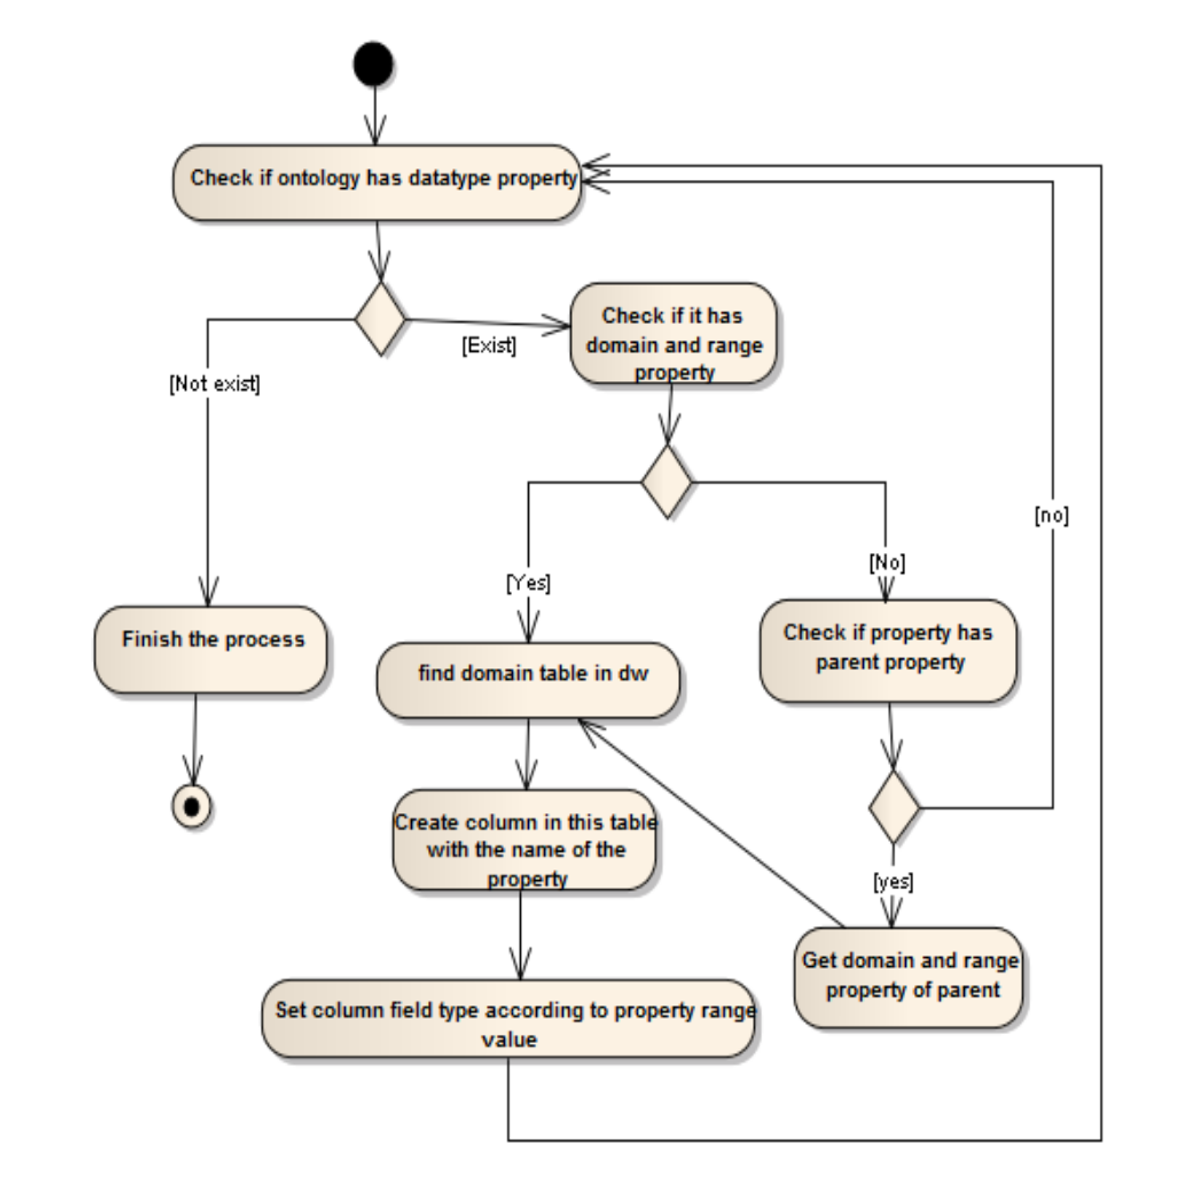
\includegraphics[scale=0.6]{data_property}
        \caption{\textbf{Cuarta etapa:} Detección de propiedades de dato} \cite[p.~21]{ontologias}.
        \label{dataProperty}
      \end{center}
    \end{figure}
    
    
    \subsubsection{Insertar datos en las tablas}
    
    En este punto es necesario enfocar la atención en los individuos de la ontología. Cada individuo se corresponde con una clase en particular, por lo tanto se
    insertará un nuevo registro (creando así un nuevo id) que será la representación del individuo en el DW. Luego, si existe alguna clase padre con respecto a la
    que se acaba de hacer el insert, se insertará un nuevo registro en la misma, el cual tendrá relacionado la clave ajena correspondiente. Como siguiente paso,
    se deben tener en cuenta las propiedades de datos. Se busca la tabla correspondiente a la clase dominio de la propiedad y se actualiza la columna que tiene el
    mismo nombre que la propiedad con el valor del rango según el individuo respectivo del dominio. En caso que no exista la clase dominio, se busca la clase
    dominio de la propiedad de datos padre. De forma similar, teniendo en vista las propiedades de objetos,  se identifica la tabla dominio (en su defecto, la 
    tabla dominio de la propiedad padre) y se actualiza la fila correspondiente al individuo de la clase dominio, en la columna con el mismo nombre que la
    propiedad, con el valor del individuo de la clase rango. En caso que no exista la columna en la tabla dominio, ésta es creada y se realiza el procedimiento
    antes descripto. El diagrama de la Figura \ref{insertingData} ilustra de forma más detallada lo recién explicado, incluyendo cada uno de los pasos a seguir.
    
    \begin{figure}[!htb]
      \begin{center}
        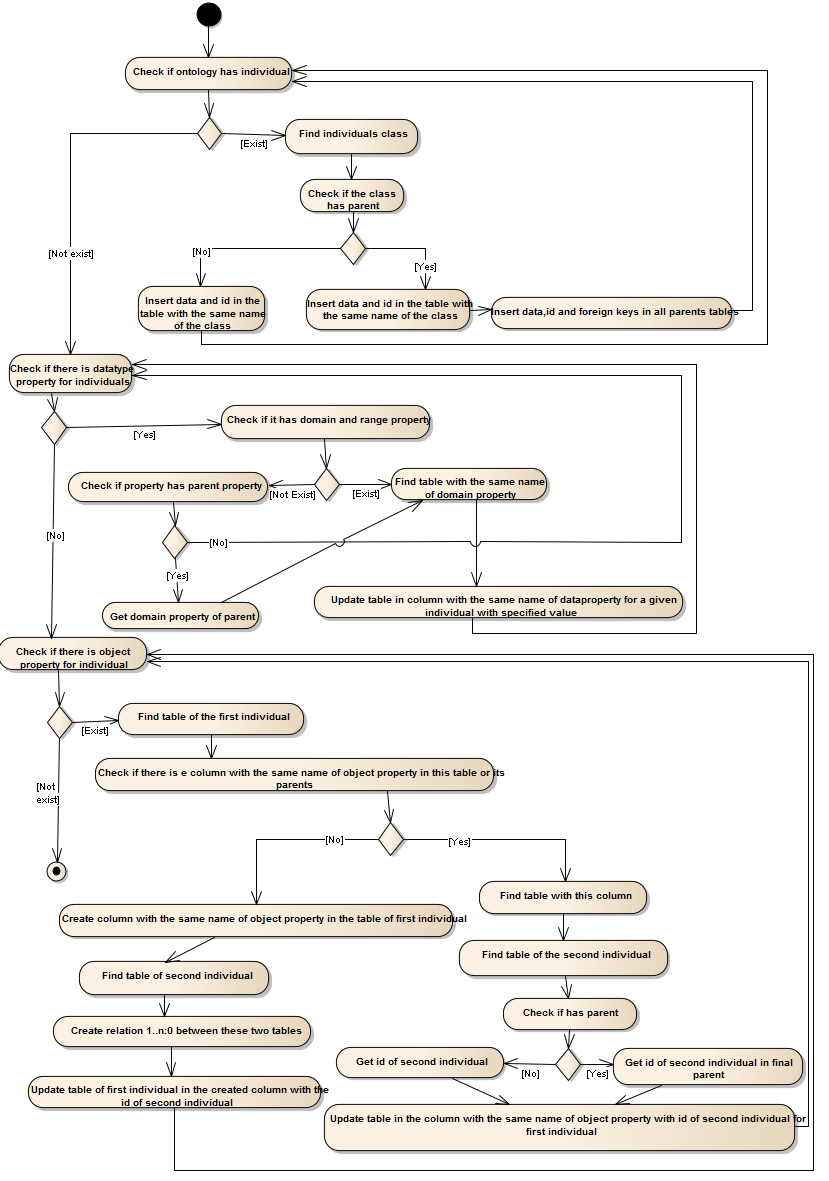
\includegraphics[scale=0.4]{inserting_data}
        \caption{\textbf{Quinta etapa:} Inserción de datos} \cite[p.~22]{ontologias}.
        \label{insertingData}
      \end{center}
    \end{figure}
    
    
    Como se puede apreciar, haciendo uso de cada una de las etapas anteriormente explicadas, se puede obtener una estructura dimensional, la cual estará
    formada por tablas de dimensiones y de hechos, a partir de datos organizados utilizando OWL. Cabe remarcar que cada una de las etapas tiene una manera
    mecánica de realizarse, con lo cual, facilita la tarea y, por otro lado, permite la automatización de ciertas partes del método utilizando algoritmos con el
    fin de simplificar aún más la labor a realizar.
    
    \subsection{Fuzzy Data Warehouse}
    
    \textbf{Fuzzy Data Warehouse} (FDW, almacén de datos difuso), es un \textit{Data Warehouse}, que contiene datos difusos, y que admite el procesamiento
    de los datos difusos.
    La incorporación de conceptos difusos, permite a los DWs, procesar los datos a mayor nivel de abstracción, y mejorar el análisis de datos imprecisos.
    
    Se trataron varios enfoques para integrar conceptos difusos en un almacén de datos y OLAP. 
    En \cite{Fasel14} se explica que la mayoría de estos enfoques han sido desarrollados para un determinado campo de aplicación, y que a menudo establecen
    restricciones en la aplicación de los conceptos difusos.
    Otras alternativas, sustituyen los valores originales del almacén de datos con datos difusos, lo que imposibilita el análisis de los valores originales del
    almacén de datos.
    
    Por ello en \cite{Fasel14}, se propone un modelo que aborda estos inconvenientes, proporcionando un método más flexible para integrar los conceptos difusos,
    utilizando \textbf{meta tablas} \footnote{Ver \ref{MFDW}.}.
    Lo que posibilita la integración de los datos difusos en cada nivel de la jerarquía de dimensiones, sin afectar la sumarización de la dimensión; donde los datos
    difusos pueden no ser normalizados. 
    Otra ventaja del modelo propuesto, es la capacidad de analizar el FDW simultáneamente en forma difuso y no difusa.
    
    \subsubsection{Lógica Difusa}
    
    Zadeh desarrolló en la teoría de conjuntos difusos un medio para representar el lenguaje natural matemáticamente. Define una \textbf{variable lingüística}, que tiene 
    palabras o frases como sus valores. Los valores de la variable lingüística, llamados \textbf{términos lingüísticos}, se proyectan sobre un universo del discurso.
    Se define a un conjunto borroso como sigue:
        
    \textbf{Conjunto difuso}. Un conjunto difuso $A$ en $M$, también llamado universo del discurso, es caracterizado por una función
    $\mu_{A}(m)$, que asocia a cada elemento en $M$, un número en el intervalo $[0,1]$. Los números en el intervalo $[0,1]$ definen la pertenencia
    de un elemento $m$ al conjunto difuso A, donde 1 implica plena pertenencia, y 0 implica ninguna pertenencia.
    
    El conjunto borroso se utilizan para definir el grado de pertenencia con la que un valor podría pertenecer a un término lingüístico.
    
    Una \textbf{variable lingüística} es una quintupla, $(X, T(X), G, M, F)$, definida como sigue:
        
    \begin{itemize}
      \item $X$ es el nombre de la variable lingüística.
      \item $T(X)$, es el conjunto de términos lingüísticos de X.
      \item $G$ es regla sintáctica que genera el conjunto de términos lingüísticos.
      \item $M$ es el universo de discurso.
      \item $F$ es una regla semántica que define para cada término lingüístico, su significado en función de un subconjunto borroso en M.
    \end{itemize}
    
    A modo de ejemplo, se tiene un conjuntos de películas, donde cada película tiene una duración específica, y se define una variable lingüística \textit{duration},
    con el siguiente conjunto de términos lingüísticos: $\{ very\,short, short, medium, long, very\,long \}$.
    En la Figura \ref{ejVarLinguistica}, se aprecia una posible representación gráfica de $duration$.
    
    \begin{figure}
      \begin{center}
        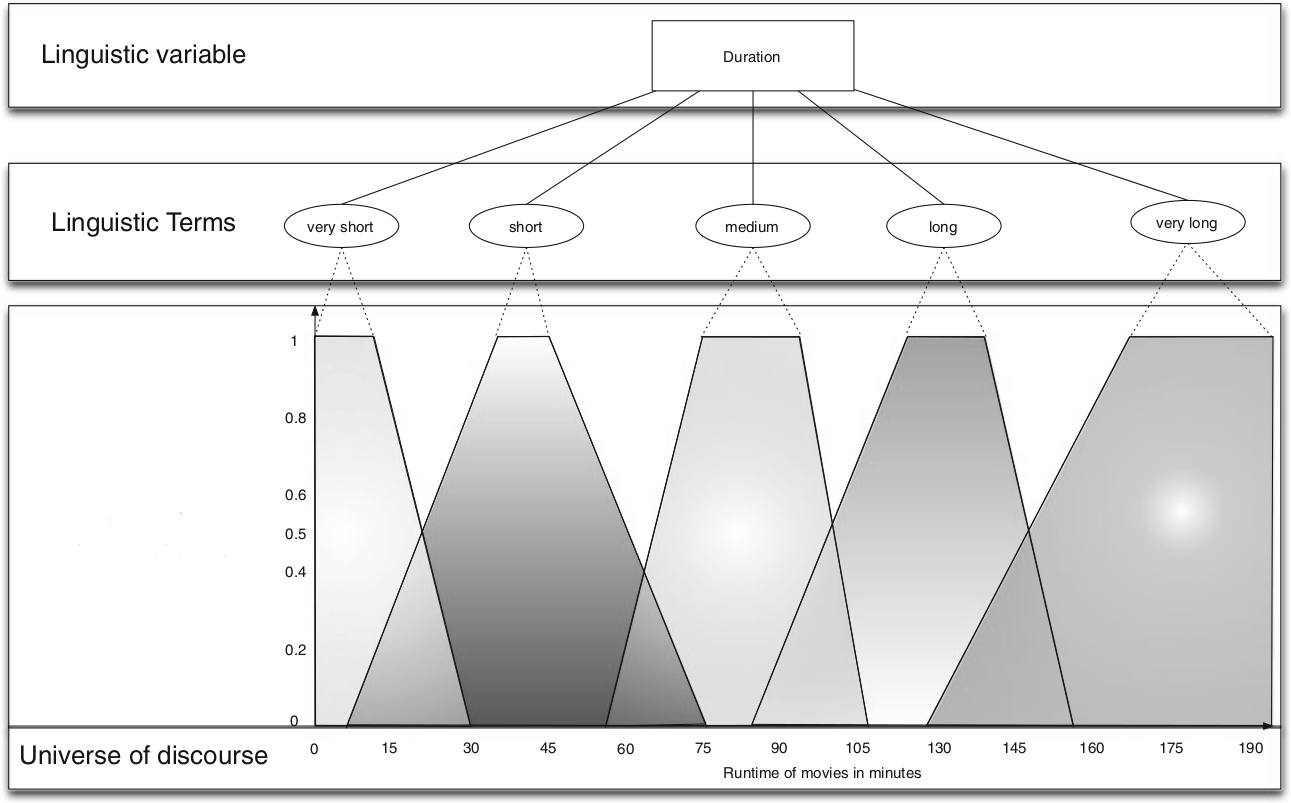
\includegraphics[scale=0.3]{fuzzy1}
        \caption{Representación gráfica de la variable lingüística $duration$. \cite[p.~39]{Fasel14}.}
        \label{ejVarLinguistica}
      \end{center}
    \end{figure}
    
    
    \subsubsection{Modelo Fuzzy Data Warehouse} \label{MFDW}
    
    A continuación se presentan los conceptos básicos del meta modelo, propuesto en \cite{Fasel14}.
    
    \begin{itemize}
    
    \item El \textbf{atributo objetivo}, lo notamos $TA$, es un atributo, de una dimensión o hecho, que quiere ser clasificado como difuso.

    \item El \textbf{atributo de pertenencia a una clase}, para un $TA$, es un atributo que tiene un conjunto de términos lingüísticos
    $T_{1},T_{2}, \ldots , T_{k}$. Lo notamos $CMA_{TA}$.
    
    \item La \textbf{función de pertenencia}, para un término lingüístico $t$ en $CMA_{TA}$, $\mu_{t} : TA \rightarrow [0,1]$,
    es utilizada para calcular los grados de pertenencia de los valores en $TA$, al término $t$.

    \item El \textbf{atributo grado de pertenencia}, de un $TA$, lo notamos $MDA_{TA}$, tiene un conjunto de grados de pertenencia del $TA$,
    para términos lingüísticos en $CMA_{TA}$.
    
    \item La \textbf{tabla de clasificación fuzzy}, $FCT$, es un tabla con dos atributos, los términos lingüísticos y sus identificadores.
    Es decir, $FCT_{TA} = \{ ID, CMA_{TA} \}$.
    
    \item La \textbf{tabla de pertenencia fuzzy}, $FMT$, es una tabla que almacena el grado, en el que los valores del $TA$,
    están relacionados con los términos lingüísticos.
    
    Es decir, $FMT_{TA} = \{ ID, ID \, de \, TA, ID \, de \, CMA_{TA}, MDA_{TA} \}$.
  
    \item El \textbf{Modelo Fuzzy Data Warehouse}, se define $FDW = \{Dim, Fact, FCT_{TA}, FMT_{TA} \}$.
    
    \end{itemize}
    
    En la Figura \ref{modeloFuzzy}, el lado izquierdo muestra cómo los conceptos fuzzy se integran con un DW clásico, mediante el uso de \textbf{meta tablas}.
    Para cada atributo objetivo es posible añadir un modelo $FDW$ .
    Por lo tanto, un DW clásico puede tener una o más meta tablas del modelo $FDW$.
    
    Además, los conceptos difusos pueden existir sin una variable lingüística. Esto es puede representar sin una tabla de clasificación fuzzy.
    Cada tabla de clasificación fuzzy tiene una relación de uno o más, con la tabla de  pertenencia fuzzy. En definitiva, el modelo $FDW$ se compone de una o más tablas
    de  pertenencia fuzzy, y cero o más tabla de clasificación fuzzy.
    
    Para proporcionar un DW funcional, el FDW tiene que apoyar las operaciones OLAP básicas. En \cite{Fasel14} se describe cómo las operaciones clásica tienen que
    adaptarse para manejar conceptos difusos correctamente, y cómo la definición del cubo de datos tiene que ser ampliada con conceptos difusos.
    
    \begin{figure}
      \begin{center}
        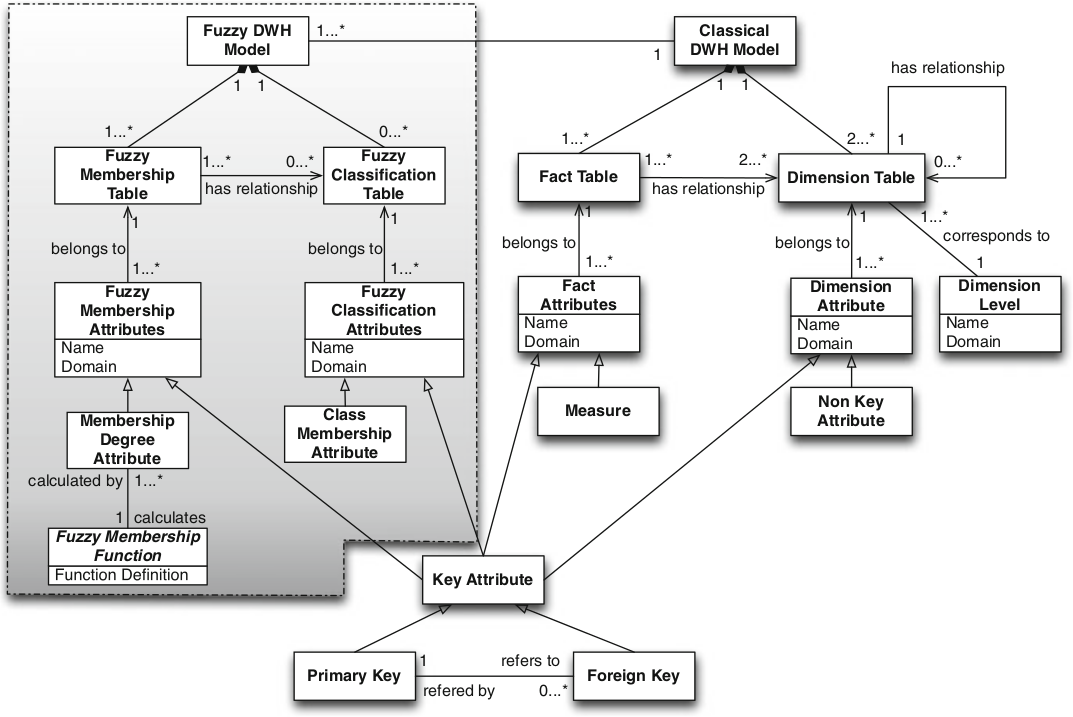
\includegraphics[scale=0.4]{fuzzy2}
        \caption{El meta modelo fuzzy data warehouse. \cite[p.~63]{Fasel14}.}
        \label{modeloFuzzy}
      \end{center}
    \end{figure}
    
    En \cite{Fasel09} se propone un Fuzzy Data Warehouse para un sistema de análisis web, donde no es posible contar las visitas de distintos usuarios con precisión.

    Se tiene una métrica (las visitas a páginas web) imprecisa. La clasificación de a los usuarios, está limita por su precisión.
    Un usuario que tiene 75 visitas podría ser clasificado como un mal visitante, mientras que un visitante con 80 visitas podría ser clasificada como buena visitante.
    A causa de la imprecisión de la métrica, un usuario podría ser clasificado en la clase equivocada. Por tanto, es difícil comparar los usuarios.
    Mediante el uso de una clasificación difusa el usuario puede pertenecer a ambos términos lingüísticos al mismo tiempo.
        
    Entonces, el concepto difuso sobre las visitas a páginas web proporciona una clasificación más certera de los valores numéricos.
    
    
    \subsection{Web Warehouse}
    
    \subsubsection{Motivación}
    
    Un \textbf{Web Warehouse} es un DW, en el cual la información es obtenida de las posibles fuentes de datos de la web. Como se menciona en \cite{webwarehouse}
    la idea de Web Warehouse es algo similar a la de un DW ya que en su arquitectura ya son bastante parecidos. La calidad de los datos es un punto crucial a la
    hora de utilizar datos provenientes de la web debido a que pueden ser poco relevantes, erróneos en sus tipos de datos, estar incompletos y tener valores
    nulos. En \cite{webwarehouse} se plantean una arquitectura y el ciclo de vida del WW con el fin de tener flexibilidad a la hora de elección de las fuentes de
    datos y llevar un buen control de los datos utilizados.
    
    
    \subsubsection{Arquitectura}
    
    La arquitectura del WW se puede dividir en algunos módulos, cada uno de ellos con tareas específicas:
    
    \begin{itemize}
      \item \textbf{Módulo DSI:} De la sigla en ingles Data Service Infrastructure (o infraestructura de servicio de datos). Este módulo tiene 3 tareas
      principales:
        \begin{itemize}
          \item Proveer un mecanismo para extraer datos de los diferentes tipos WDS (Web Data Source o, su traducción al castellano, fuentes de datos web) y
          mostrarlos a todos ellos como DS homogéneos (Data Service o servicio de datos). Los DS son los encargados de acceder y extraer la información de la web.
          \item Monitorear los DS y periódicamente controlar la calidad de los datos que ingresan. Estos controles son realizados por ciertos DS que son
          invocados por el móludo QM (Quality Measurement o de medición de calidad) e incluyen el almacenamiento de metadatos de DQ (Data Quality o calidad de
          datos) y QoS (Quality of Service o calidad de servicio).
          \item Provee mecanismos para reaccionar ante la degradación de un DS, ya que si ésto sucede, los datos perderán relevancia.
        \end{itemize}
      \item \textbf{Módulo integrador:} Este módulo lleva a cabo la integración de datos y provee los mismos en un formato normalizado, construyendo con ellos la
      IDB (Integrated Data Base o base de datos integrada). Sus principales objetivos son la selección de los DS con el fin de obtener calidad en los datos
      extraidos de la web, integración de datos y la generación de metadatos de esos datos integrados.
      \item \textbf{Módulos ETL y OLAP:} Estos módulos realizan las tareas usuales salvo que deben propagar los metadatos de la calidad de datos.
      \item \textbf{Módulo DWQM:} Es la sigla para Data Warehouse Quality Measurement ó medición de calidad del DW. Como lo indica su nombre, es el módulo
      encargado de medir la calidad de los datos del DW.
    \end{itemize}
    
    Las conexiones entre los distintos módulos pueden ser observadas en la Figura \ref{ww_arq}, donde se puede apreciar claramente la propagación entre de los
    metadatos (punto destacado en la explicación de los módulos).
    
    \begin{figure}[!htb]
      \begin{center}
        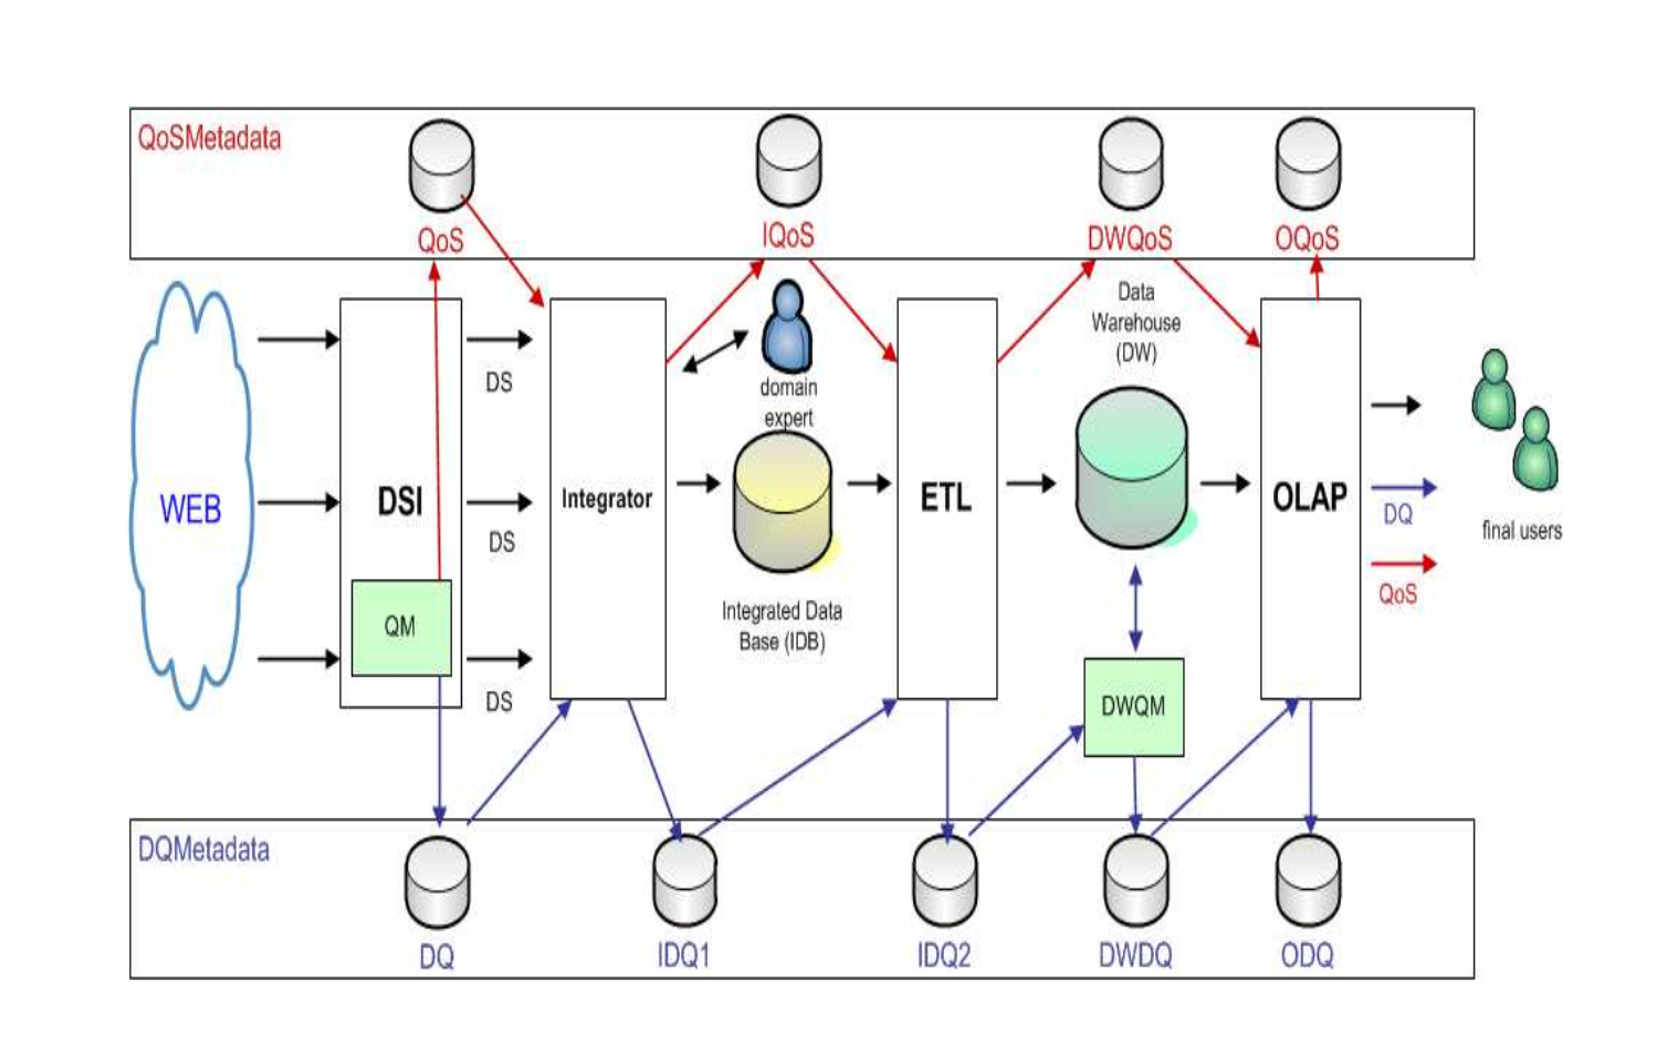
\includegraphics[scale=0.25]{ww_arq}
        \caption{Arquitectura genérica de un Web Warehouse} \cite[p.~2]{webwarehouse}.
        \label{ww_arq}
      \end{center}
    \end{figure}
    
    
    \subsubsection{Ciclo de vida de un WW}
    
    El ciclo de vida de un WW, está compuesto por distintas etapas y en el se presentan los roles de las personas que participan en cada una. Las
    etapas son las que se muestran en la Figura \ref{lifecycle} y detalladas a continuación:
    
    \begin{figure}[!htb]
      \begin{center}
        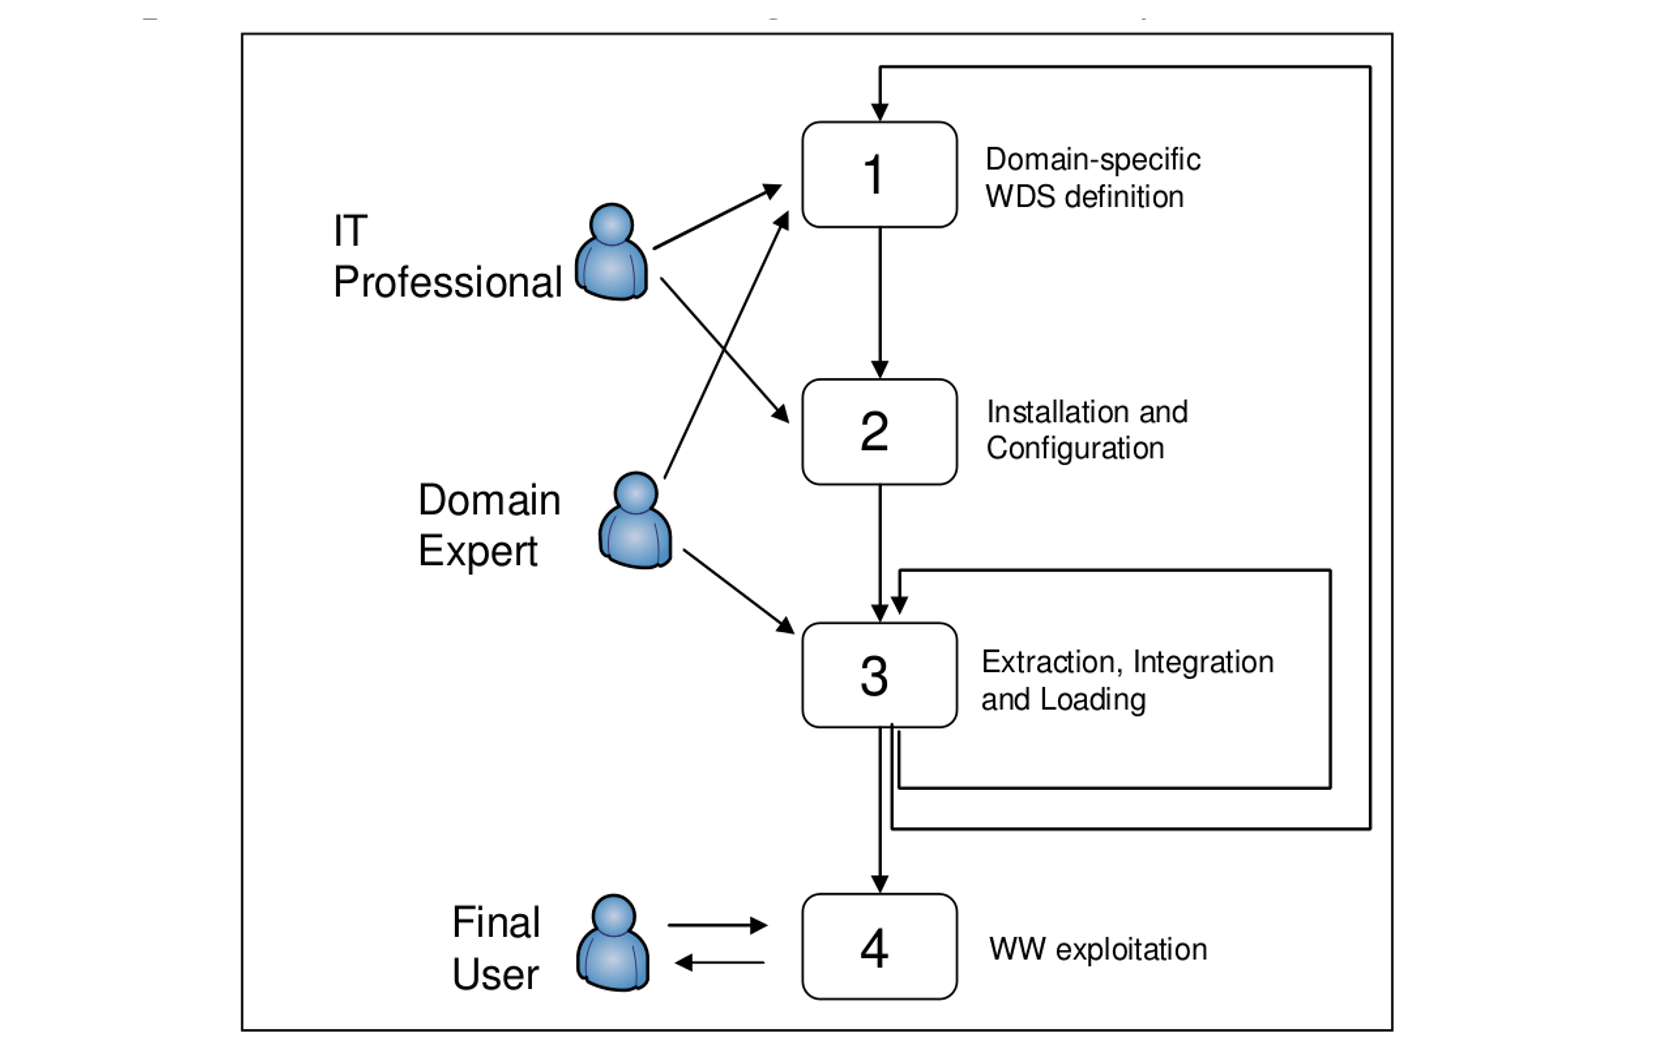
\includegraphics[scale=0.25]{lifecycle}
        \caption{Ciclo de vida de un Web Warehouse} \cite[p.~3]{webwarehouse}.
        \label{lifecycle}
      \end{center}
    \end{figure}
    
    \begin{enumerate}
      \item En este paso se elige las fuentes de datos web específicas para el dominio en el que se está trabajando, teniendo en cuenta la calidad de las mismas.
      Estas fuentes se llaman WDS seleccionadas.
      \item La siguiente instancia es donde se hacen la instalación y configuración de la plataforma para el dominio determinado dependiendo de sus
      requerimientos. Consiste en las siguientes tareas:
        \begin{enumerate}
          \item Diseño y definición del DW, lo que incluye el esquema del mismo y los procesos ETL
          \item Diseño del esquema del DSI
          \item Desarrollo de los DS
          \item Selección de los DS
        \end{enumerate}
      \item Aquí es donde se da la extracción, integración, transformación y carga de datos controlando la calidad de los mismos. En esta etapa es cuando los
      datos se toman de la web, pasan a través del sistema y cargan el DW. Como se ve en la Figura \ref{lifecycle}, desde esta etapa se puede volver a la
      primera, lo cual puede darse en el caso que se quisiera agregar una nueva fuente de datos como pueden ser nuevos sitios web. La calidad de los datos sigue
      siendo de vital importancia.
      \item Esta etapa es en la que se realiza la explotación de los datos por el usuario final.
    \end{enumerate}
    
    
    \subsubsection{Calidad de datos}
    
    Como se ha estado mencionando, la calidad de los datos es uno de los puntos más importantes en la arquitectura de un WW, ya que es la que define la calidad
    de toda la solución de negocios que se está ofreciendo al cliente u organización. Para que el lector tenga una idea más concreta sobre la calidad de los
    datos se plantean 6 factores que, a juzgar por los autores, engloban todos los aspectos referentes al tema, los cuales son:
    
    \begin{itemize}
      \item \textbf{Precisión:} Sintáctica y semánticamente correctos.
      \item \textbf{Completitud:} Cuan densos son los datos, es decir, cuanto cubren de todo lo que se necesita.
      \item \textbf{Frescura:} Periodicidad con que se cargan los datos, límite de tiempo luego del cual los datos dejan de ser válidos.
      \item \textbf{Consistencia:} Los datos deben ser consistentes respecto del dominio en que se trabaja.
      \item \textbf{Unicidad:} No debe haber duplicidad en los datos.
      \item \textbf{Confiabilidad:} Los datos deben tener credibilidad y ser objetivos.
    \end{itemize}
  
  % ############################ FIN ESTADO DEL ARTE ############################
  
  % ############################ INICIO CONCLUSIONES ############################

  \section{Conclusiones} \label{conclusiones}
  
  Se puede observar que la aplicación del modelo dimensional sobre el Data Warehouse, junto con las diversas formas de explotación de los datos, entre ellas
  OLAP \footnote{Ver Figura \ref{dw_arq}.}, ofrece una solución que ayuda al usuario final en la toma de decisiones, respaldando las mismas con resultados concretos.
  
  La principal ventaja del enfoque dimensional, en contraposición al modelo normalizado, es el desarrollo de estructuras fáciles de entender y usar para el
  usuario final. Si se siguiera una normalización en tercera forma normal, debido al gran número de tablas que se crearían, podría ser engorroso para el
  usuario establecer los joins necesarios, sobre las distintas fuentes de datos, que provean de información significativa, sin una comprensión plena
  de las estructuras de datos del Data Warehouse.
  Además, tiende a proporcionar de una mayor performance, en la recuperación de los datos, gracias al grado de desnormalización de los datos.
  
  Por otro lado, se considera importante remarcar que las herramientas OLAP se adaptan mejor, en escenarios donde se requiera de tomas de decisiones,
  que las herramientas OLTP, debido a sus diferentes naturalezas.
  Los DWs están optimizados para patrones de búsquedas analíticos, que en general consisten en la selección de campos determinados, que requieren de pocos
  \texttt{``select *''}.
  
  A diferencias de las bases de datos operacionales que mantienen una fotografía del estado
  de la organización, los DWs mantienen datos históricos, que se implementa a través de procesos ETL, los cuales migran periódicamente los datos de los sistemas
  operacionales al Data Warehouse.
  
  En referencia al uso de ontologías aplicadas al diseño del DW, publicado en \cite{ontologias}, es importante aclarar que, si bien cada uno de los pasos del
  algoritmo están bien diferenciados y detallados, no se explica como distinguir las dimensiones y los hechos de manera explícita, a partir de las clases
  que componen la ontología resultante de aplicar el algoritmo. Por lo tanto, éste tema está abierto a futuras investigaciones.
  
  Daniel Fasel, en \cite {Fasel14}, destaca que el modelo de Fuzzy Data Warehouse, se basa en un enfoque relacional del DW.
  Por ello, es necesario analizar en futuras investigaciones si la estructura de la tabla meta puede ser implementada en bases de datos multidimensionales,
  o si sería necesaria una nueva implementación de los conceptos difusos.
  Además, la estructura de meta tablas no contempla ningún control de versiones cronológico de datos difusos.
  Es decir que, no es posible tener diferentes versiones de datos borrosos en diferentes puntos del tiempo.
  
  % Saqué información de https://en.wikipedia.org/wiki/Data_warehouse.
  % De la sección "Dimensional vs. normalized approach for storage of data" y "Data warehouses versus operational systems".

  % ############################ FIN CONCLUSIONES ############################

  % ############################ INICIO BIBLIOGRAFIA ############################
  \section{Bibliografia}

  \printbibliography

  % ############################ FIN BIBLIOGRAFIA ############################
  
  
  \printindex %?
  
\end{document}
